%%%%%%%%%%%%%%%%%%%%%%%%%%%%%%%%%%%%%%%%%
% Masters/Doctoral Thesis
% LaTeX Template
% Version 2.5 (27/8/17)
%
% This template was downloaded from:
% http://www.LaTeXTemplates.com
%
% Version 2.x major modifications by:
% Vel (vel@latextemplates.com)
%
% This template is based on a template by:
% Steve Gunn (http://users.ecs.soton.ac.uk/srg/softwaretools/document/templates/)
% Sunil Patel (http://www.sunilpatel.co.uk/thesis-template/)
%
% Template license:
% CC BY-NC-SA 3.0 (http://creativecommons.org/licenses/by-nc-sa/3.0/)
%
%%%%%%%%%%%%%%%%%%%%%%%%%%%%%%%%%%%%%%%%%

%----------------------------------------------------------------------------------------
%	PACKAGES AND OTHER DOCUMENT CONFIGURATIONS
%----------------------------------------------------------------------------------------

\documentclass[
11pt, % The default document font size, options: 10pt, 11pt, 12pt
%oneside, % Two side (alternating margins) for binding by default, uncomment to switch to one side
english, % ngerman for German
singlespacing, % Single line spacing, alternatives: onehalfspacing or doublespacing
%draft, % Uncomment to enable draft mode (no pictures, no links, overfull hboxes indicated)
%nolistspacing, % If the document is onehalfspacing or doublespacing, uncomment this to set spacing in lists to single
%liststotoc, % Uncomment to add the list of figures/tables/etc to the table of contents
%toctotoc, % Uncomment to add the main table of contents to the table of contents
%parskip, % Uncomment to add space between paragraphs
%nohyperref, % Uncomment to not load the hyperref package
headsepline, % Uncomment to get a line under the header
%chapterinoneline, % Uncomment to place the chapter title next to the number on one line
%consistentlayout, % Uncomment to change the layout of the declaration, abstract and acknowledgements pages to match the default layout
]{MastersDoctoralThesis} % The class file specifying the document structure

\usepackage[utf8]{inputenc} % Required for inputting international characters
\usepackage[T1]{fontenc} % Output font encoding for international characters

\usepackage{mathpazo} % Use the Palatino font by default

\usepackage[backend=bibtex,style=authoryear,natbib=true]{biblatex} % Use the bibtex backend with the authoryear citation style (which resembles APA)

\addbibresource{main.bib} % The filename of the bibliography

\usepackage[autostyle=true]{csquotes} % Required to generate language-dependent quotes in the bibliography

%----------------------------------------------------------------------------------------
%	MARGIN SETTINGS
%----------------------------------------------------------------------------------------

\geometry{
	paper=a4paper, % Change to letterpaper for US letter
	inner=2.5cm, % Inner margin
	outer=3.8cm, % Outer margin
	bindingoffset=.5cm, % Binding offset
	top=1.5cm, % Top margin
	bottom=1.5cm, % Bottom margin
	%showframe, % Uncomment to show how the type block is set on the page
}

%----------------------------------------------------------------------------------------
%	THESIS INFORMATION
%----------------------------------------------------------------------------------------

\thesistitle{Thesis Title} % Your thesis title, this is used in the title and abstract, print it elsewhere with \ttitle
\supervisor{Dr. James \textsc{Smith}} % Your supervisor's name, this is used in the title page, print it elsewhere with \supname
\examiner{} % Your examiner's name, this is not currently used anywhere in the template, print it elsewhere with \examname
\degree{Doctor of Philosophy} % Your degree name, this is used in the title page and abstract, print it elsewhere with \degreename
\author{John \textsc{Smith}} % Your name, this is used in the title page and abstract, print it elsewhere with \authorname
\addresses{} % Your address, this is not currently used anywhere in the template, print it elsewhere with \addressname

\subject{Biological Sciences} % Your subject area, this is not currently used anywhere in the template, print it elsewhere with \subjectname
\keywords{} % Keywords for your thesis, this is not currently used anywhere in the template, print it elsewhere with \keywordnames
\university{\href{http://www.university.com}{University Name}} % Your university's name and URL, this is used in the title page and abstract, print it elsewhere with \univname
\department{\href{http://department.university.com}{Department or School Name}} % Your department's name and URL, this is used in the title page and abstract, print it elsewhere with \deptname
\group{\href{http://researchgroup.university.com}{Research Group Name}} % Your research group's name and URL, this is used in the title page, print it elsewhere with \groupname
\faculty{\href{http://faculty.university.com}{Faculty Name}} % Your faculty's name and URL, this is used in the title page and abstract, print it elsewhere with \facname

\AtBeginDocument{
\hypersetup{pdftitle=\ttitle} % Set the PDF's title to your title
\hypersetup{pdfauthor=\authorname} % Set the PDF's author to your name
\hypersetup{pdfkeywords=\keywordnames} % Set the PDF's keywords to your keywords
}

\begin{document}

\frontmatter % Use roman page numbering style (i, ii, iii, iv...) for the pre-content pages

\pagestyle{plain} % Default to the plain heading style until the thesis style is called for the body content

%----------------------------------------------------------------------------------------
%	TITLE PAGE
%----------------------------------------------------------------------------------------

\begin{titlepage}
\begin{center}

\vspace*{.06\textheight}
{\scshape\LARGE \univname\par}\vspace{1.5cm} % University name
\textsc{\Large Doctoral Thesis}\\[0.5cm] % Thesis type

\HRule \\[0.4cm] % Horizontal line
{\huge \bfseries \ttitle\par}\vspace{0.4cm} % Thesis title
\HRule \\[1.5cm] % Horizontal line

\begin{minipage}[t]{0.4\textwidth}
\begin{flushleft} \large
\emph{Author:}\\
\href{http://www.johnsmith.com}{\authorname} % Author name - remove the \href bracket to remove the link
\end{flushleft}
\end{minipage}
\begin{minipage}[t]{0.4\textwidth}
\begin{flushright} \large
\emph{Supervisor:} \\
\href{http://www.jamessmith.com}{\supname} % Supervisor name - remove the \href bracket to remove the link
\end{flushright}
\end{minipage}\\[3cm]

\vfill

\large \textit{A thesis submitted in fulfillment of the requirements\\ for the degree of \degreename}\\[0.3cm] % University requirement text
\textit{in the}\\[0.4cm]
\groupname\\\deptname\\[2cm] % Research group name and department name

\vfill

{\large \today}\\[4cm] % Date
%\includegraphics{Logo} % University/department logo - uncomment to place it

\vfill
\end{center}
\end{titlepage}

%----------------------------------------------------------------------------------------
%	DECLARATION PAGE
%----------------------------------------------------------------------------------------

\begin{declaration}
\addchaptertocentry{\authorshipname} % Add the declaration to the table of contents
\noindent I, \authorname, declare that this thesis titled, \enquote{\ttitle} and the work presented in it are my own. I confirm that:

\begin{itemize}
\item This work was done wholly or mainly while in candidature for a research degree at this University.
\item Where any part of this thesis has previously been submitted for a degree or any other qualification at this University or any other institution, this has been clearly stated.
\item Where I have consulted the published work of others, this is always clearly attributed.
\item Where I have quoted from the work of others, the source is always given. With the exception of such quotations, this thesis is entirely my own work.
\item I have acknowledged all main sources of help.
\item Where the thesis is based on work done by myself jointly with others, I have made clear exactly what was done by others and what I have contributed myself.\\
\end{itemize}

\noindent Signed:\\
\rule[0.5em]{25em}{0.5pt} % This prints a line for the signature

\noindent Date:\\
\rule[0.5em]{25em}{0.5pt} % This prints a line to write the date
\end{declaration}

\cleardoublepage

%----------------------------------------------------------------------------------------
%	QUOTATION PAGE
%----------------------------------------------------------------------------------------

\vspace*{0.2\textheight}

\noindent\enquote{\itshape Thanks to my solid academic training, today I can write hundreds of words on virtually any topic without possessing a shred of information, which is how I got a good job in journalism.}\bigbreak

\hfill Dave Barry

%----------------------------------------------------------------------------------------
%	ABSTRACT PAGE
%----------------------------------------------------------------------------------------

\begin{abstract}
\addchaptertocentry{\abstractname} % Add the abstract to the table of contents
The Thesis Abstract is written here (and usually kept to just this page). The page is kept centered vertically so can expand into the blank space above the title too\ldots
\end{abstract}

%----------------------------------------------------------------------------------------
%	ACKNOWLEDGEMENTS
%----------------------------------------------------------------------------------------

\begin{acknowledgements}
\addchaptertocentry{\acknowledgementname} % Add the acknowledgements to the table of contents
The acknowledgments and the people to thank go here, don't forget to include your project advisor\ldots
\end{acknowledgements}

%----------------------------------------------------------------------------------------
%	LIST OF CONTENTS/FIGURES/TABLES PAGES
%----------------------------------------------------------------------------------------

\tableofcontents % Prints the main table of contents

\listoffigures % Prints the list of figures

\listoftables % Prints the list of tables

%----------------------------------------------------------------------------------------
%	ABBREVIATIONS
%----------------------------------------------------------------------------------------

\begin{abbreviations}{ll} % Include a list of abbreviations (a table of two columns)

\textbf{LAH} & \textbf{L}ist \textbf{A}bbreviations \textbf{H}ere\\
\textbf{WSF} & \textbf{W}hat (it) \textbf{S}tands \textbf{F}or\\

\end{abbreviations}

%----------------------------------------------------------------------------------------
%	PHYSICAL CONSTANTS/OTHER DEFINITIONS
%----------------------------------------------------------------------------------------

\begin{constants}{lr@{${}={}$}l} % The list of physical constants is a three column table

% The \SI{}{} command is provided by the siunitx package, see its documentation for instructions on how to use it

Speed of Light & $c_{0}$ & \SI{2.99792458e8}{\meter\per\second} (exact)\\
%Constant Name & $Symbol$ & $Constant Value$ with units\\

\end{constants}

%----------------------------------------------------------------------------------------
%	SYMBOLS
%----------------------------------------------------------------------------------------

\begin{symbols}{lll} % Include a list of Symbols (a three column table)

$a$ & distance & \si{\meter} \\
$P$ & power & \si{\watt} (\si{\joule\per\second}) \\
%Symbol & Name & Unit \\

\addlinespace % Gap to separate the Roman symbols from the Greek

$\omega$ & angular frequency & \si{\radian} \\

\end{symbols}

%----------------------------------------------------------------------------------------
%	DEDICATION
%----------------------------------------------------------------------------------------

\dedicatory{For/Dedicated to/To my\ldots}

%----------------------------------------------------------------------------------------
%	THESIS CONTENT - CHAPTERS
%----------------------------------------------------------------------------------------

\mainmatter % Begin numeric (1,2,3...) page numbering

\pagestyle{thesis} % Return the page headers back to the "thesis" style

% Include the chapters of the thesis as separate files from the Chapters folder
% Uncomment the lines as you write the chapters

% Chapter 1: Introduction

\chapter{Introducción} % Main chapter title

\label{Chapter1} % For referencing the chapter elsewhere, use \ref{Chapter1}

%----------------------------------------------------------------------------------------

% Define some commands to keep the formatting separated from the content
\newcommand{\keyword}[1]{\textbf{#1}}
\newcommand{\tabhead}[1]{\textbf{#1}}
\newcommand{\code}[1]{\texttt{#1}}
\newcommand{\file}[1]{\texttt{\bfseries#1}}
\newcommand{\option}[1]{\texttt{\itshape#1}}

%----------------------------------------------------------------------------------------

\section{Motivación}

Es de sobra conocida la importantica de la analítica de datos en nuestro tiempo, así también lo es la referida al desarrollo de \emph{software}\index{software}. Herramientas como GrimoireLab\index{GrimoireLab} posibilitan este fin.

Para acercar su uso a perfiles no técnicos, los creadores de GrimoireLab\index{GrimoireLab} idearon Cauldron\index{Cauldron}, un SaaS de GrimoireLab que funciona como una aplicación web. Con un par de clics, un usuario es capaz de poner en marcha el sistema y obtener datos referidos al desarrollo de \emph{software}\index{software} fácilmente.

Sin embargo, esta plataforma no está exenta de defectos. Como parte del equipo desarrollador de Cauldron\index{Cauldron}, el autor de este Trabajo de Fin de Máster conoce de primera mano los puntos de mejora del sistema.

Con este pretexto comienza el desarrollo de una herramienta que facilite la analítica de datos referente al desarrollo de \emph{software}\index{software}, soslayando las dificultades encontradas durante el desarrollo de Cauldron\index{Cauldron}.

%----------------------------------------------------------------------------------------

\section{Estructura de la memoria}

La estructura que esta memoria sigue es la siguiente:

\begin{itemize}
    \item En el Capítulo~\ref{Chapter2} se explican varios conceptos y tecnologías que ya existen y que se han usado para llevar a cabo el proyecto.
    \item En el Capítulo~\ref{Chapter3} se detalla el desarrollo del proyecto, desde el trabajo previo al comienzo del proyecto hasta los problemas encontrados durante el desarrollo, pasando por los diferentes prototipos de la aplicación.
    \item En el Capítulo~\ref{Chapter4} se exponen las especificaciones del sistema final, incluyendo instrucciones detalladas para poner la aplicación en funcionamiento, así como un caso de uso.
    \item En el Capítulo~\ref{Chapter5} se finaliza la memoria haciendo una reflexión sobre los resultados y las posibles líneas de desarrollo futuras.
\end{itemize}

%----------------------------------------------------------------------------------------

\section{Objetivos}

\subsection{Objetivo general}

El objetivo principal de este proyecto es el desarrollo de una plataforma similar a Cauldron\index{Cauldron}, que permita el análisis de ecosistemas de desarrollo de \emph{software}\index{software}, modificando algunas partes de su funcionamiento original, añadiendo nuevas características, y resolviendo varios problemas que el proyecto original llevaba arrastrando desde su comienzo.

\subsection{Objetivos específicos}

Para llevar a cabo el objetivo principal del proyecto, se han elaborado una serie de objetivos más específicos:

\begin{itemize}
    \item El esquema de funcionamiento en Cauldron\index{Cauldron} gira en torno a la generación de informes alterables, esto es, cuando un usuario analiza una o varias fuentes de datos es capaz de modificar (incluso cuando el análisis no ha finalizado) la lista de objetos a analizar. De la misma manera, un informe realizado hace meses continúa actualizando los datos mostrados si otro usuario (o el creador) lo solicita. Esta característica, si bien permitía no tener que analizar varias veces un mismo repositorio para tener datos actualizados, generaba bastantes problemas de desarrollo al tener que lidiar con múltiples factores que podían alterar los datos de un informe. Uno de los objetivos que persigue este proyecto es que la nueva plataforma genere informes inalterables, creando un flujo más simple desde la solicitud por parte del usuario al \emph{output} de la aplicación.
    \item Muchos de los servicios que componen Cauldron\index{Cauldron} tienen una fuerte dependencia entre ellos, de manera que el fallo en uno puede ocasionar el fallo general del sistema. En un entorno en el que el desarrollo \emph{serverless} y las arquitecturas basadas en microservicios son cada vez más frecuentes, es necesaria la creación de sistemas desacoplados que funcionen en su conjunto para dar un servicio. Este proyecto persigue el desarrollo de varios componentes \emph{software}\index{software} independientes que colaboren entre ellos para dar un servicio al usuario.
    \item Cauldron\index{Cauldron} utiliza GrimoireLab\index{GrimoireLab} (más concretamente la herramienta conocida como SirMordred) para realizar las tareas de recogida y enriquecimiento de datos. La forma en la que Cauldron opera con la herramienta es mediante un contenedor Docker\index{Docker} personalizado, el cual deriva de uno proporcionado por GrimoireLab, lo que añade más complejidad al incluir un componente extra que necesita ser mantenido. Este objetivo pretende simplificar el uso de GrimoireLab mediante la ejecución del contenedor Docker original de GrimoireLab. Aparte, otro de los componentes de GrimoireLab, llamado Sorting Hat, añade limitaciones al sistema (o complejidad, según se mire) al ser requisito inalterable para su funcionamiento el uso de una base de datos MariaDB. Debido a esto, y a que el RGPD\footnote{Reglamento General de Protección de Datos} limita el valor que se le puede dar a una plataforma como esta, se ha decidido eliminar este componente del esquema de la nueva plataforma.
    \item El último objetivo que busca este proyecto está relacionado con mejoras menores respecto a Cauldron\index{Cauldron}, como el uso de Poetry\index{Poetry} para la gestión de dependencias, la sustitución del servidor WSGI de Django\index{Django} por Gunicorn\index{Gunicorn}, o la detección de actualizaciones de dependencias con Dependabot\index{Dependabot}.
\end{itemize}

% Chapter 2: State of the Art

\chapter{Tecnologías utilizadas} % Main chapter title

\label{Chapter2} % For referencing this chapter elsewhere, use \ref{Chapter2}

%-------------------------------------------------------------------------------

\section{Python\index{Python}}

Python\index{Python} es un lenguaje de programación orientada a objetos de alto nivel. Fue desarrollado originalmente por Guido van Rossum en el final de la década de 1980, y actualmente es gestionado por la \emph{Python Software Foundation} bajo una licencia \emph{open source}\index{open source} propia conocida como PSFL (\emph{Python Software Foundation License}). \emph{\parencite{Reference1}}

\begin{figure}[ht]
    \centering
    
\includegraphics[width=0.3\textwidth]{Figures/python-logo}
    \decoRule
    \caption[Python (Logo)]{Logo de Python\index{Python} \emph{\parencite{Reference2}}}
    \label{fig:python-logo}
\end{figure}

Python\index{Python} es actualmente uno de los lenguajes de programación más populares. Esto se debe en gran parte a su modularidad, la cual permite agregar fácilmente nuevas piezas de código a aplicaciones ya desarrolladas. \emph{\parencite{Reference3}}

\subsection{Poetry}

Poetry\index{Poetry} es un gestor de paquetes y dependencias para Python\index{Python}. Entre sus características más destacadas se encuentra la generación de un fichero con la especificación exacta de dependencias (incluidas las dependencias de dependencias), lo que asegura instalaciones idénticas en diferentes entornos. \emph{\parencite{Reference6}}

Además de esto, Poetry\index{Poetry} incorpora la mayoría de reglas establecidas en PEP\footnote{PEP (\emph{Python Enhancement Proposal}) recoge y describe las principales guías y recomendaciones de la comunidad respecto a nuevas características y procesos para cualquier desarrollo con Python.}, como el uso del fichero \emph{pyproject.toml} para escribir la metainformación de los paquetes, o el uso del esquema \emph{major.minor.micro} para los identificadores de versión. \emph{\parencite{Reference6}}

%-------------------------------------------------------------------------------

\section{HTTP}

\emph{Hypertext Transfer Protocol} (HTTP\index{HTTP}) es un protocolo de nivel de aplicación para sistemas de información distribuidos.

Es un protocolo genérico y sin estado que es usado para múltiples tareas como la transferencia de hipertexto o la representación de sistemas de ficheros.

Una característica de HTTP\index{HTTP} es la negociación de la representación de los datos, lo que permite construir sistemas independientemente de los datos que se vayan a transmitir. \emph{\parencite{Reference26}}

\subsection{API REST}

Una API\index{API} (\emph{Application Programming Interface}) es un contrato entre dos equipos sobre como deben comunicarse entre ellos. Con el uso de APIs se pretende abstraer los detalles acerca de como un sistema funciona internamente, haciendo públicas solo aquellas partes que los desarrolladores pudieran encontrar interesantes. De hecho, aunque la lógica interna cambiara, la API debería permanecer intacta. \emph{\parencite{Reference27}}

REST\index{REST} (\emph{Representational State Transfer}) es un estilo de arquitecura \emph{software}\index{software} para sistemas distribuidos que operan con contenido de diverso tipo. La idea tras este estilo es que cada respuesta del servidor debe ser una representación de un recurso (comúnmente en formato JSON\index{JSON}), siendo las llamadas a este solicitudes para la creación, actualización o eliminación de un recurso. \emph{\parencite{Reference28}}

Por tanto, una API\index{API} REST\index{REST} sería aquella que sigue los principios arquitectónicos que le dan nombre.

%-------------------------------------------------------------------------------

\section{Django}\label{sec:django}

Django\index{Django} es un \emph{web framework} desarrollado para Python\index{Python} y que, al igual que este, cuenta con una licencia \emph{open source}\index{open source}. Fue desarrollado originalmente por Adrian Holovaty y Simon Willison, dos programadores web que trabajaban en un periódico. \emph{\parencite{Reference4}}

\begin{figure}[ht]
    \centering
    
\includegraphics[width=0.3\textwidth]{Figures/django-logo}
    \decoRule
    \caption[Django (Logo)]{Logo de Django\index{Django} \emph{\parencite{Reference5}}}
    \label{fig:django-logo}
\end{figure}

Django\index{Django} sigue los principios de modularidad que caracterizan a Python\index{Python}, además de incluir muchas otras características interesantes como un sistema de vistas, modelos y plantillas que permite agilizar el desarrollo de aplicaciones web. Esto, sumado a un servidor web simple para desarrollos locales, una interfaz administrativa intuitiva, y la posibilidad de construir \emph{middleware} de todo tipo, convierten a Django\index{Django} en uno de los \emph{frameworks} para desarrollo web más famosos y usados de los últimos años. \emph{\parencite{Reference4}}

\subsection{Django REST Framework}

Django\index{Django} REST Framework (DRF) es un módulo para Django que amplía las características de este, y que facilita la creación de APIs REST manteniendo todas las ventajas de Django. \emph{\parencite{Reference7}}

\begin{figure}[ht]
    \centering
    
\includegraphics[width=0.5\textwidth]{Figures/drf-logo}
    \decoRule
    \caption[DRF (Logo)]{Logo de DRF \emph{\parencite{Reference8}}}
    \label{fig:drf-logo}
\end{figure}

A diferencia del \emph{framework} original, DRF se centra principalmente en la parte \emph{backend} que compone una aplicación web. Para ello, ofrece al usuario muchas más opciones para serializar la entrada y salida de datos, además de ampliar las conocidas \emph{Generic Views} de Django con mejoras relacionadas con la construcción de APIs. \emph{\parencite{Reference7}}

Permite además interaccionar fácilmente con la API construida a través de una interfaz web básica, y es capaz de generar documentación dinámica para la API siguiendo la especificación de OpenAPI\footnote{\url{https://spec.openapis.org/oas/v3.1.0}}. \emph{\parencite{Reference7}}

\subsection{Gunicorn}\label{sec:gunicorn}

Gunicorn\index{Gunicorn} (\emph{"Green Unicorn"}) es un servidor HTTP\index{HTTP}, escrito en Python\index{Python}, que implementa WSGI\footnote{WSGI (\emph{Web Server Gateway Interface}) establece cómo deben ser llevadas las peticiones del servidor web a la aplicación web escrita en Python, de manera síncrona. \emph{\parencite{Reference11}}} como protocolo de llamadas.

Funciona utilizando un esquema centralizado, donde un nodo maestro gestiona y orquesta diferentes tipos de nodos trabajadores. Estos pueden ser utilizados para procesar peticiones síncronas o asíncronas, y su número escala en función de la demanda que tenga el servidor. \emph{\parencite{Reference9}}

\begin{figure}[ht]
    \centering
    
\includegraphics[width=0.4\textwidth]{Figures/gunicorn-logo}
    \decoRule
    \caption[Gunicorn (Logo)]{Logo de Gunicorn \emph{\parencite{Reference10}}}
    \label{fig:gunicorn-logo}
\end{figure}

%-------------------------------------------------------------------------------

\section{GrimoireLab}\label{sec:grimoirelab}

GrimoireLab\index{GrimoireLab} es el resultado de años de investigación y análisis de comunidades \emph{open source}\index{open source} y procesos de desarrollo. Desarrollado originalmente por miembros del equipo \emph{LibreSoft} (que más tarde fundarían Bitergia), actualmente forma parte de CHAOSS, una iniciativa de la \emph{Linux Foundation} centrada en crear y modelar métricas sobre comunidades \emph{open source}\index{open source}. \emph{\parencite{Reference12}}

\begin{figure}[ht]
    \centering
    
\includegraphics[width=0.2\textwidth]{Figures/grimoirelab-logo}
    \decoRule
    \caption[GrimoireLab (Logo)]{Logo de GrimoireLab \emph{\parencite{Reference12}}}
    \label{fig:grimoirelab-logo}
\end{figure}

Se trata de un conjunto de herramientas diseñadas para recoger, enriquecer, consumir y visualizar datos de casi cualquier fuente relacionada con el desarrollo \emph{Open Source}\index{open source}.

Cada una de estas herramientas sirve a un propósito específico y, en su conjunto, proveen el servicio antes mencionado:

\begin{itemize}
    \item Perceval es el encargado de recoger los datos crudos de cada fuente de datos compatible con GrimoireLab\index{GrimoireLab}. Ya sea utilizando herramientas como Git\index{Git} o haciendo uso de la API\index{API} de la fuente analizada.
    \item GrimoireELK enriquece los datos recogidos por Perceval. Genera, a partir de estos, nuevos datos que son de interés para estudiar las comunidades \emph{open source}\index{open source}.
    \item Sorting Hat permite gestionar la información relacionada con identidades, incluso entre diferentes fuentes de datos.
    \item SirMordred es la herramienta orquestadora para GrimoireLab\index{GrimoireLab}. Se encarga de sincronizar a todas las componentes para dar servicio.
    \item ¡Y muchas más herramientas increíbles!
\end{itemize}

\begin{figure}[ht]
    \centering
    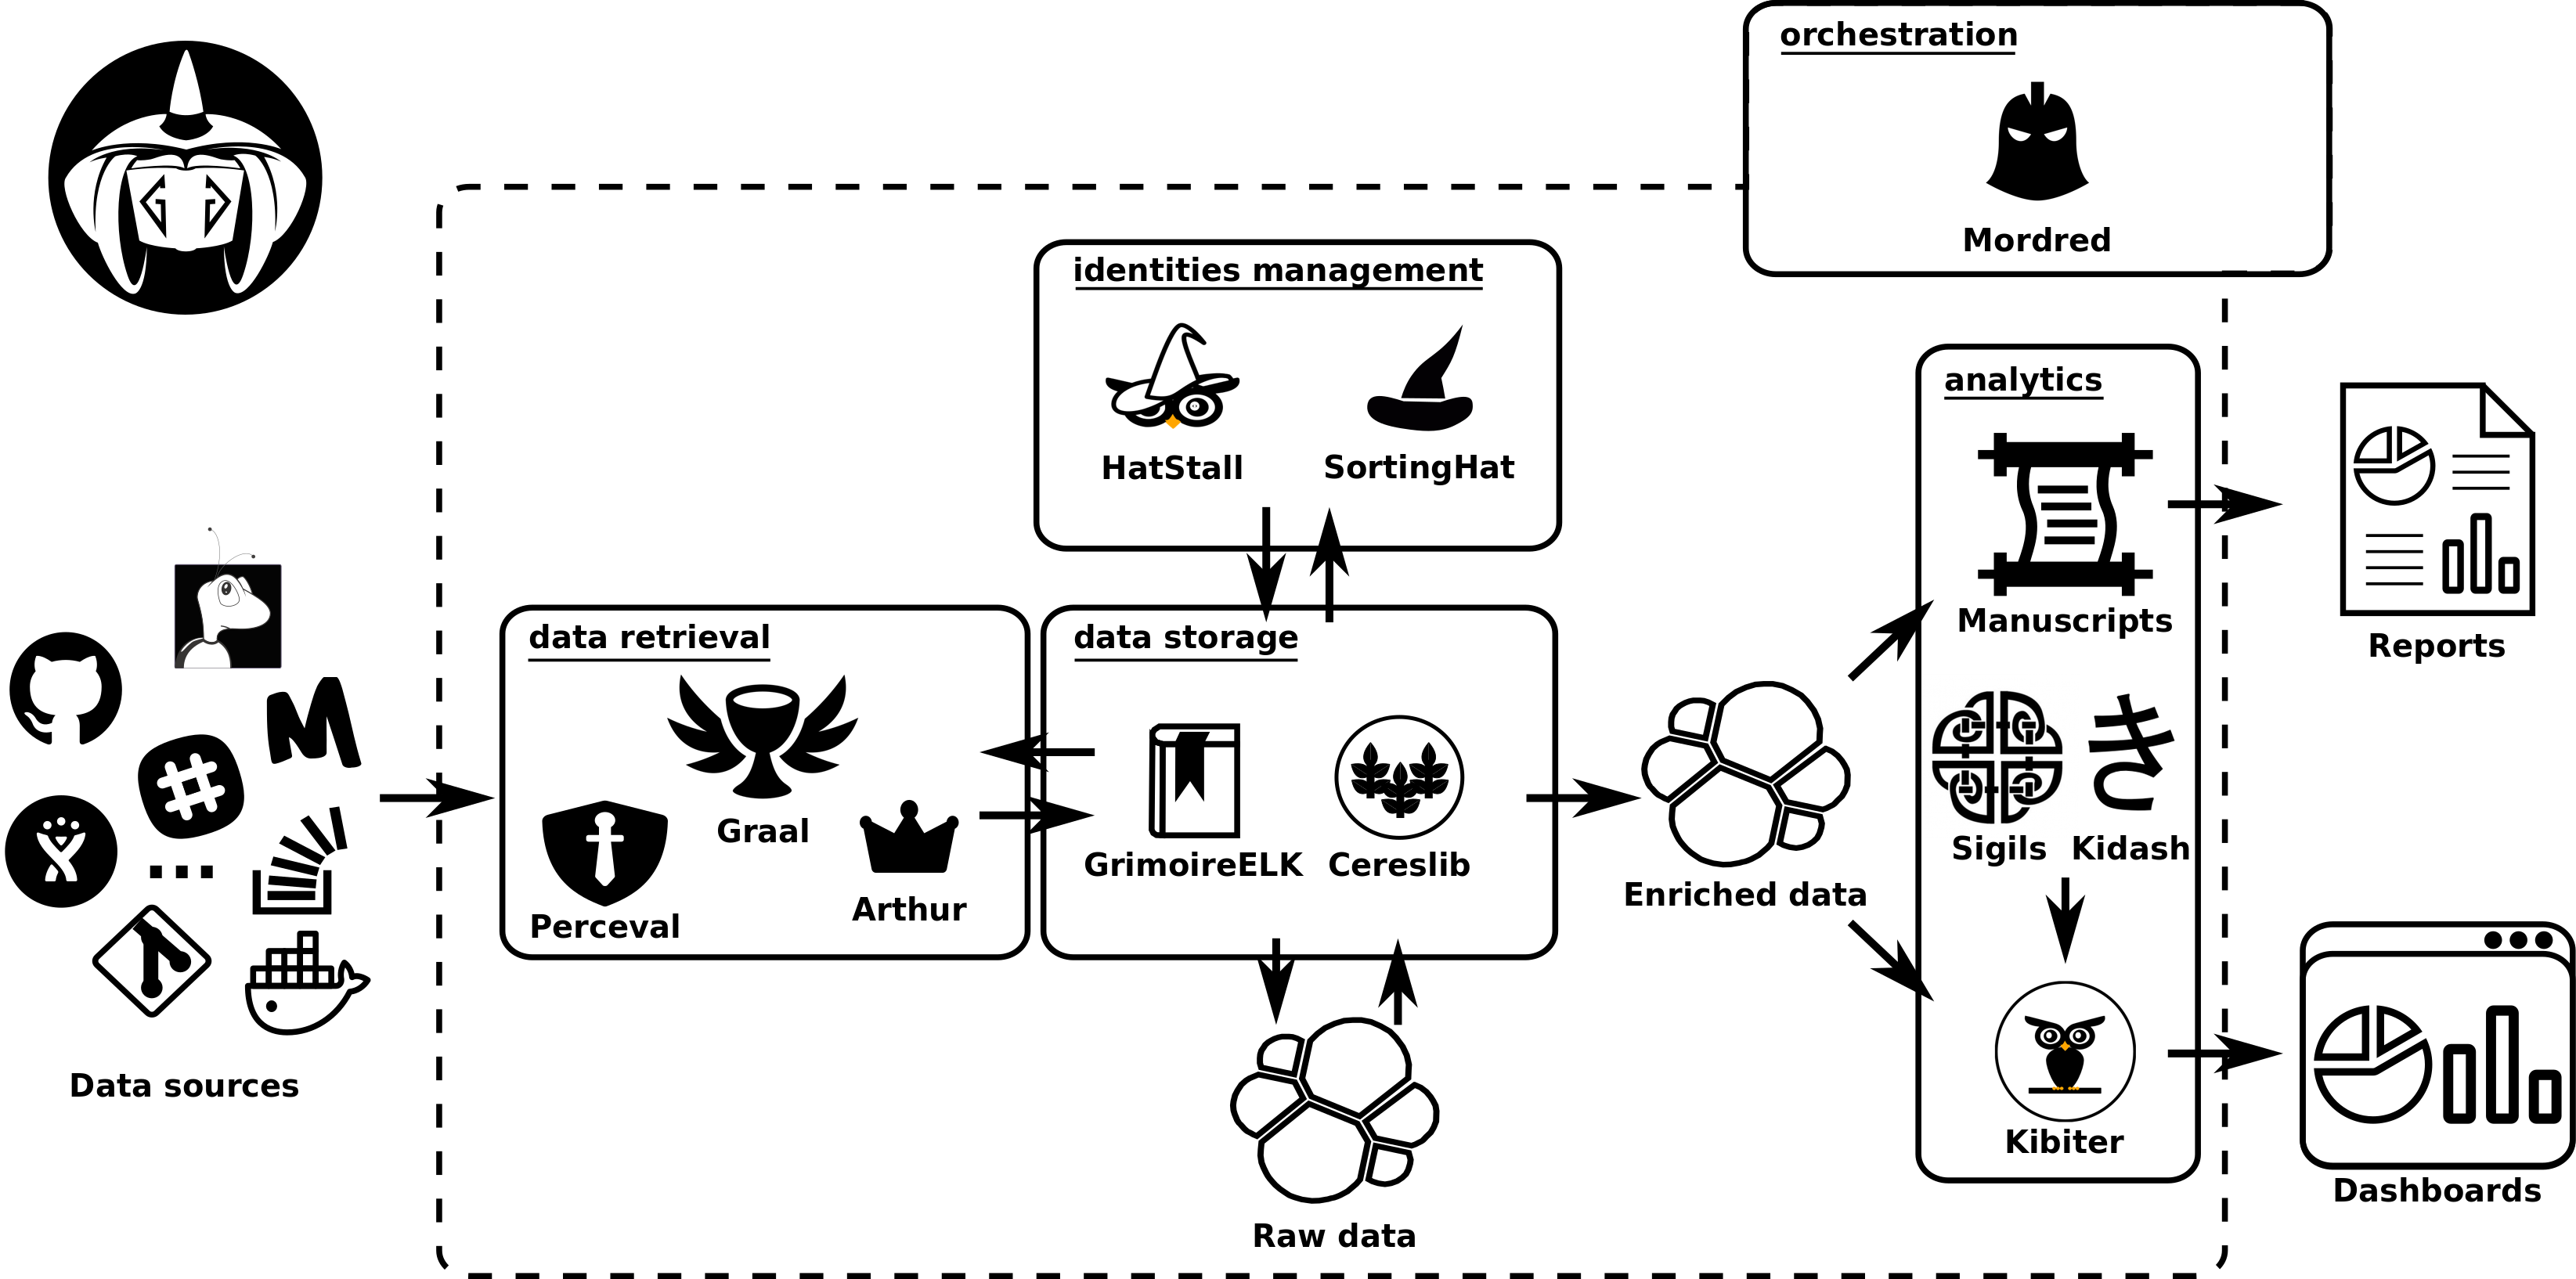
\includegraphics[width=0.7\textwidth]{Figures/grimoirelab-schema}
    \decoRule
    \caption[GrimoireLab (Esquema)]{Esquema de GrimoireLab \emph{\parencite{Reference12}}}
    \label{fig:grimoirelab-schema}
\end{figure}

\subsection{Cauldron.io}

Cauldron.io (o simplemente Cauldron\index{Cauldron}) es una plataforma web que permite a sus usuarios utilizar GrimoireLab\index{GrimoireLab} de manera sencilla y rápida, necesitando únicamente un navegador web para su uso. \emph{\parencite{Reference13}}

\begin{figure}[ht]
    \centering
    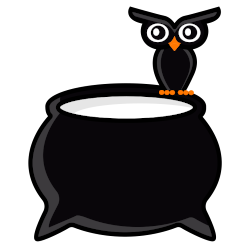
\includegraphics[width=0.2\textwidth]{Figures/cauldron-logo}
    \decoRule
    \caption[Cauldron (Logo)]{Logo de Cauldron \emph{\parencite{Reference13}}}
    \label{fig:cauldron-logo}
\end{figure}

Cauldron\index{Cauldron} nace como un SaaS\footnote{\emph{Software as a Service}} de GrimoireLab\index{GrimoireLab}, y actualmente tiene compatibilidad con algunas de las fuentes de datos más importantes dentro de los ecosistemas \emph{open source}\index{open source}, como GitHub, Meetup, o StackExchange. Está compuesto por una aplicación Django\index{Django} detrás de un servidor Nginx, y utiliza Open Distro for Elasticsearch\index{Elasticsearch} y Kibana\index{Kibana} para almacenar y visualizar los datos generados con GrimoireLab\index{GrimoireLab}, respectivamente.

\begin{figure}[ht]
    \centering
    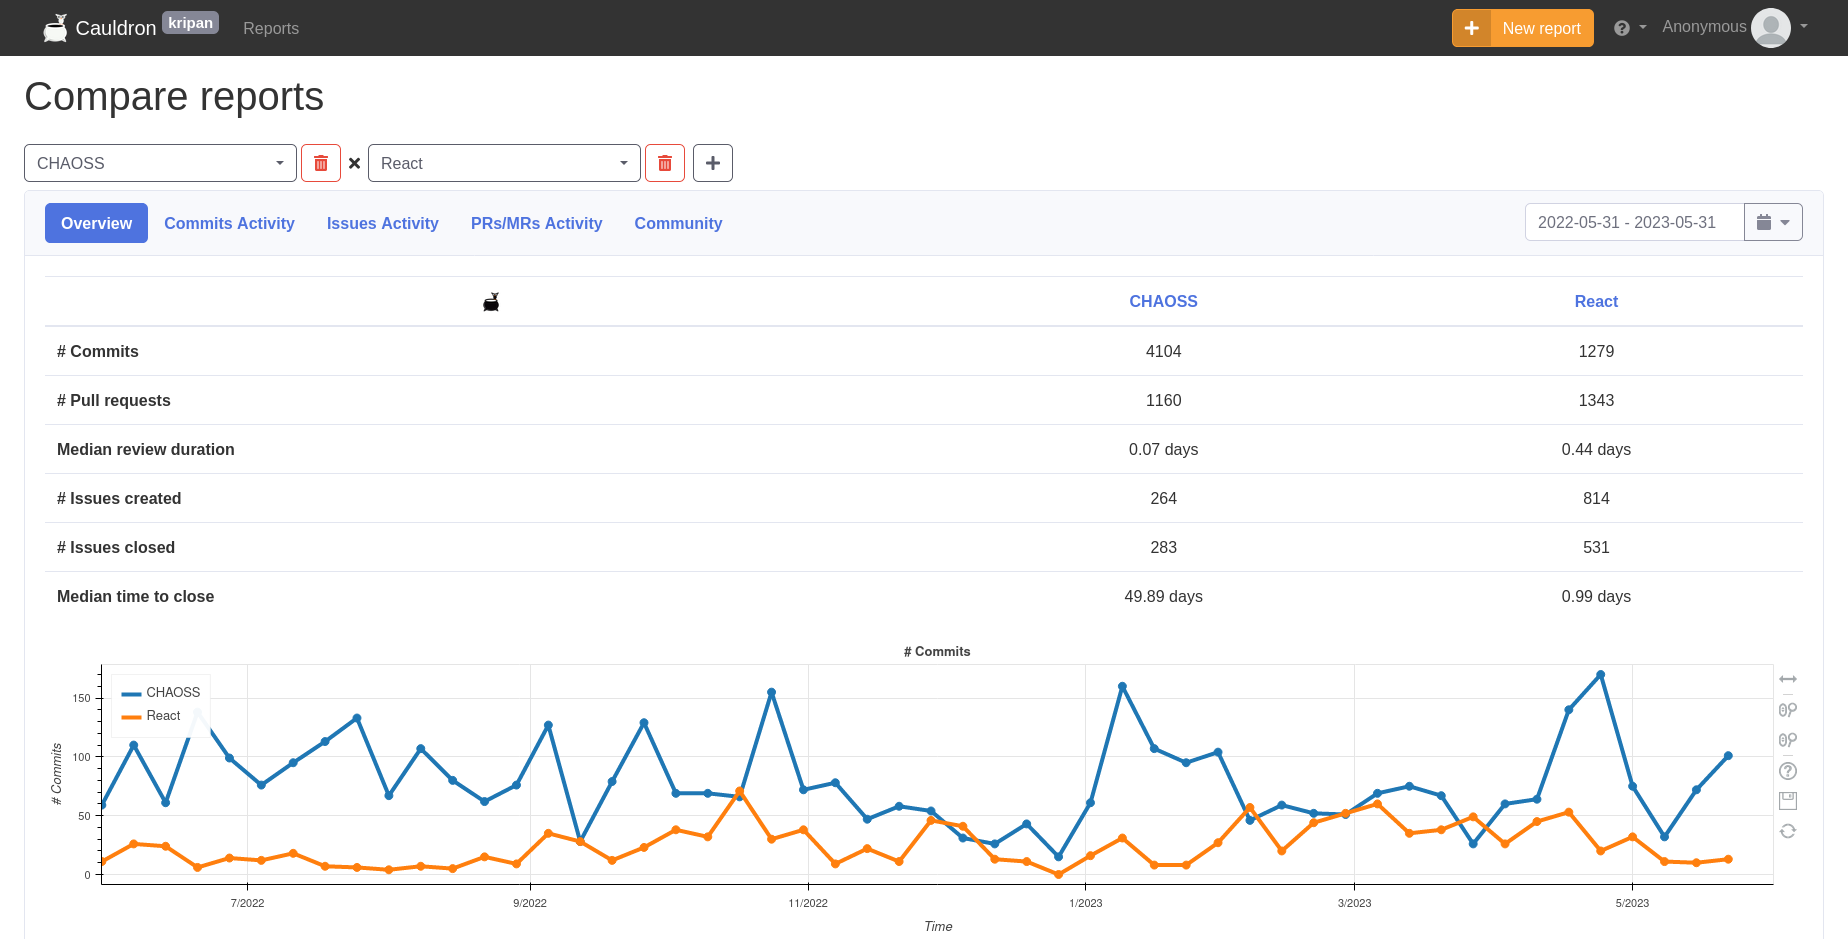
\includegraphics[width=\textwidth]{Figures/cauldron-charts}
    \decoRule
    \caption[Cauldron (Gráficas)]{Gráficas en Cauldron \emph{\parencite{Reference13}}}
    \label{fig:cauldron-charts}
\end{figure}

Además de las visualizaciones generadas en Kibana\index{Kibana}, Cauldron\index{Cauldron} ofrece a sus usuarios otras formas de dar valor a sus análisis. Como se observa en la Figura~\ref{fig:cauldron-charts}, permite comparar métricas y gráficas de diferentes proyectos. Además de esto, permite generar gráficas personalizadas dentro de Kibana\index{Kibana} gracias a las funcionalidades extra de Open Distro for Elasticsearch\index{Elasticsearch}.

%-------------------------------------------------------------------------------

\section{FastAPI}

FastAPI\index{FastAPI} es un \emph{web framework} desarrollado para Python\index{Python}, orientado principalmente a la construcción de APIs utilizando las anotaciones de tipos estándar de Python\index{Python}. \emph{\parencite{Reference14}}

\begin{figure}[ht]
    \centering
    
\includegraphics[width=0.7\textwidth]{Figures/fastapi-logo}
    \decoRule
    \caption[FastAPI (Logo)]{Logo de FastAPI \emph{\parencite{Reference14}}}
    \label{fig:fastapi-logo}
\end{figure}

FastAPI\index{FastAPI} nace después de que su autor no pudiera cubrir las necesidades de sus proyectos personales con los \emph{web frameworks} actuales en ese momento. Después de investigar las especificaciones de OpenAPI\index{OpenAPI}, JSON\index{JSON}, OAuth2, etc., decide construir su propia solución teniendo como base Pydantic\footnote{Pydantic es una herramienta que permite aprovechar las anotaciones de Python para informar de errores en la validación de datos.} y Starlette\footnote{Starlette es un framework que permite construir servicios web asíncronos en Python.}. \emph{\parencite{Reference15}}

FastAPI\index{FastAPI} hace uso de las anotaciones de tipos en Python\index{Python} para conseguir \emph{parsing} y validación de datos, documentación automática, y soporte en editores (comprobación de errores, autocompletado, etc). Hace uso de ASGI\footnote{ASGI (\emph{Asynchronous Server Gateway Interface}) es similar a WSGI, pero para llamadas asíncronas.} para llamadas asíncronas por defecto, es compatible con la mayoría de bases de datos relacionales y no relacionales, y permite tener un servicio web funcional en pocos pasos. \emph{\parencite{Reference14}}

\subsection{Uvicorn}

Uvicorn\index{Uvicorn} es un servidor HTTP\index{HTTP}, para aplicaciones Python\index{Python}, que procesa las llamadas de manera asíncrona implementando ASGI. En combinación con \nameref{sec:gunicorn}\index{Gunicorn}, se obtiene un servidor asíncrono multi nodo. \emph{\parencite{Reference16}}

\begin{figure}[ht]
    \centering
    
\includegraphics[width=0.3\textwidth]{Figures/uvicorn-logo}
    \decoRule
    \caption[Uvicorn (Logo)]{Logo de Uvicorn \emph{\parencite{Reference16}}}
    \label{fig:uvicorn-logo}
\end{figure}

%-------------------------------------------------------------------------------

\section{OpenSearch}\label{sec:opensearch}

OpenSearch\index{OpenSearch} es un \emph{suite} de herramientas \emph{open source}\index{open source} que permite el almacenamiento, búsqueda, y análisis de datos. Se trata de un proyecto formado principalmente por dos componentes: el propio motor OpenSearch\index{OpenSearch} y OpenSearch Dashboards, siendo estos un \emph{fork}\footnote{Uno de los principales motivos de su creación fue la decisión de modificar la licencia de Elasticsearch y Kibana a una no \emph{open source} por parte de sus creadores.} de los proyectos Elasticsearch\index{Elasticsearch} y Kibana\index{Kibana}, respectivamente. \emph{\parencite{Reference17}}

\begin{figure}[ht]
    \centering
    
\includegraphics[width=0.5\textwidth]{Figures/opensearch-logo}
    \decoRule
    \caption[OpenSearch (Logo)]{Logo de OpenSearch \emph{\parencite{Reference17}}}
    \label{fig:opensearch-logo}
\end{figure}

OpenSearch\index{OpenSearch} está basado en el motor de búsqueda Apache Lucene, lo que le confiere una gran capacidad de indexación en volúmenes de datos grandes. Muchas de las características que definen a OpenSearch\index{OpenSearch} provienen de plugins para Elasticsearch\index{Elasticsearch}, pero que el primero integra de manera nativa. Entre estas características destacan:

\begin{itemize}
    \item Un módulo avanzado de seguridad que permite la autenticación de usuarios mediante \emph{Active Directory}, LDAP, y otros protocolos similares. Igualmente, permite mayor granularidad sobre los permisos en índices y otras estructuras de datos.
    \item Un módulo de gestión de índices, con el que definir políticas y automatismos en índices.
    \item Un analizador de eficiencia que es capaz de obtener diversas métricas del \emph{cluster} de OpenSearch\index{OpenSearch} asociadas a la eficiencia, como la cantidad de memoria utilizada por los nodos, o el número de operaciones de lectura y escritura.
    \item Un sistema de alertas que permite establecer límites en gráficas y métricas, los cuales envían una notificación al ser rebasados.
\end{itemize}

\subsection{OpenSearch Dashboards}

OpenSearch\index{OpenSearch} Dashboards es la herramienta de visualización de datos de OpenSearch. Está basado en Kibana\index{Kibana}, tratándose de hecho de un \emph{fork} de esta. \emph{\parencite{Reference18}}

\begin{figure}[ht]
    \centering
    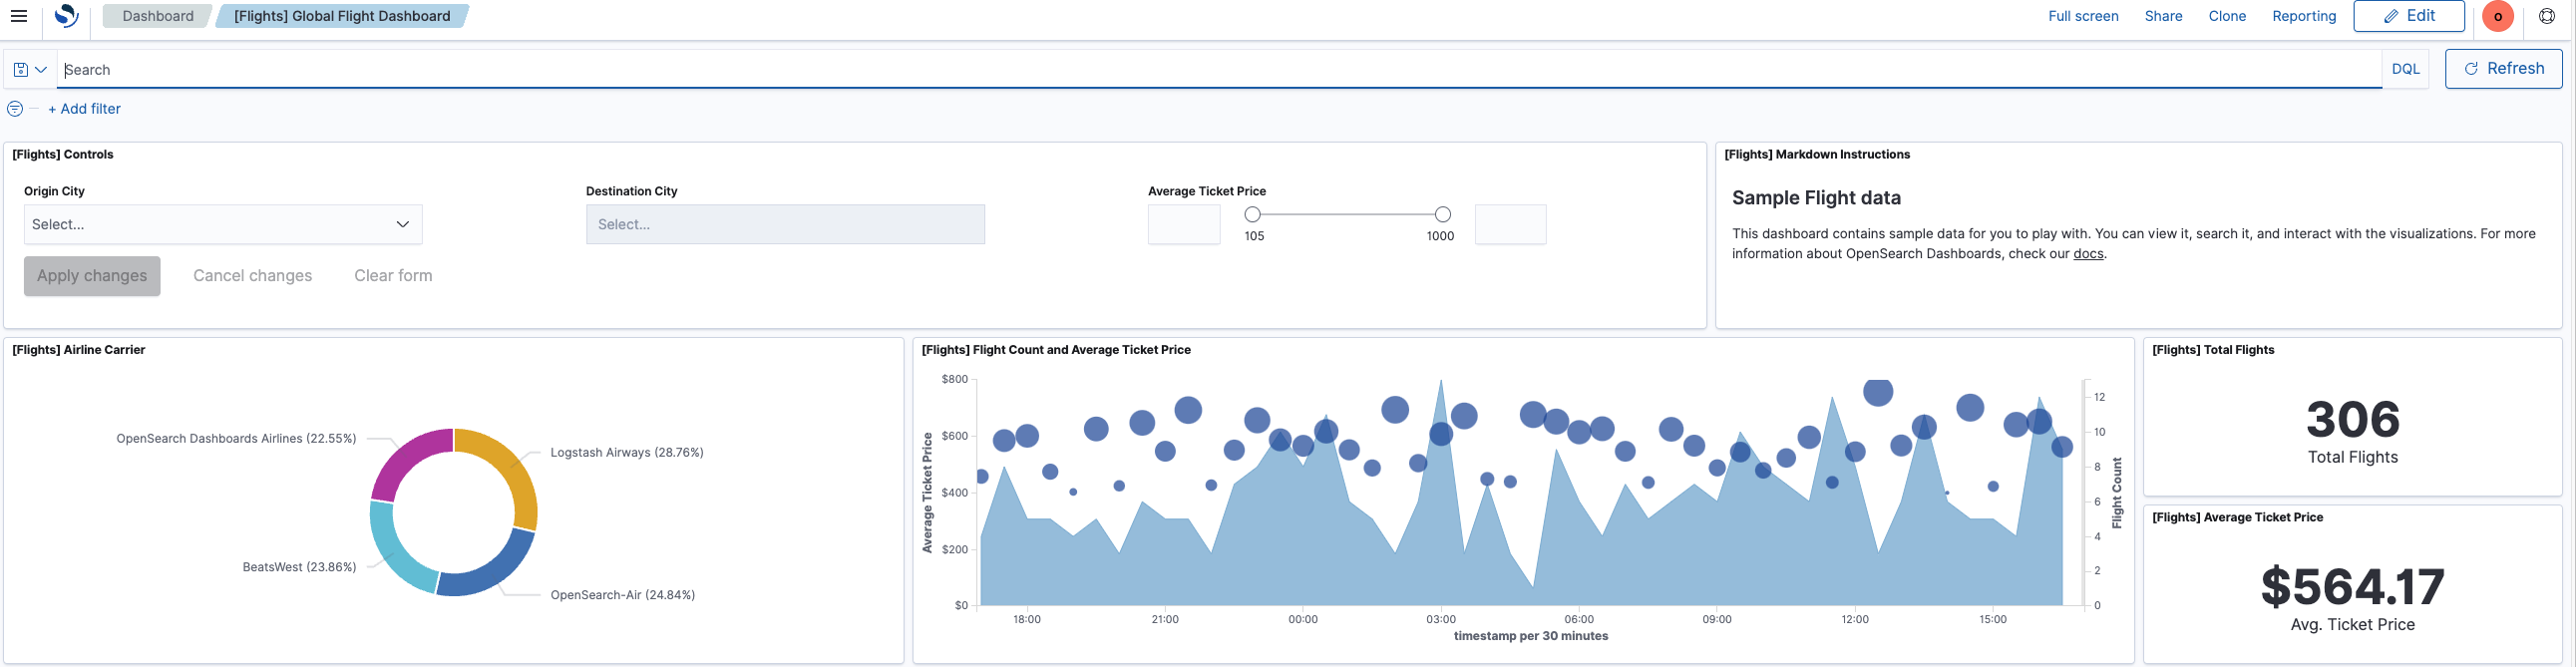
\includegraphics[width=\textwidth]{Figures/opensearch-dashboards}
    \decoRule
    \caption[OpenSearch Dashboards]{OpenSearch Dashboards \emph{\parencite{Reference18}}}
    \label{fig:opensearch-dashboards}
\end{figure}

Posee varias herramientas para interaccionar con los datos almacenados en el \emph{cluster} y crear, con estos, gráficos y métricas como los que aparecen en la Figura~\ref{fig:opensearch-dashboards}. Permite también la construcción de alias y patrones para índices, y la visualización de los datos directamente en formato JSON (tal y como están almacenados en el \emph{cluster}).

%-------------------------------------------------------------------------------

\section{PostgreSQL}

PostgreSQL\index{PostgreSQL} es un sistema de base de datos relacional con mucha historia (fue desarrollado originalmente en 1996). Cuenta con licencia \emph{open source}\index{open source}, y está gestionado por una comunidad colaborativa de desarroladores conocida como \emph{PostgreSQL Global Development Group}. \emph{\parencite{Reference19}}

\begin{figure}[ht]
    \centering
    
\includegraphics[width=0.3\textwidth]{Figures/postgresql-logo}
    \decoRule
    \caption[PostgreSQL (Logo)]{Logo de PostgreSQL \emph{\parencite{Reference19}}}
    \label{fig:postgresql-logo}
\end{figure}

PostgreSQL\index{PostgreSQL} es la opción recomendada para \nameref{sec:django}\index{Django}. Esto es debido a las muchas características que lo hacen una opción interesante, como la diversidad de estructuras nativas (\emph{arrays}, direcciones IP, etc), su capacidad para alta concurrencia, o la posibilidad de ejecutar bloques de código en el servidor.

%-------------------------------------------------------------------------------

\section{Docker}

Docker\index{Docker} es el sistema gestor de contenedores\index{Contenedor} más utilizado actualmente, debido a la sencillez de su uso y a la cantidad de funcionalidades que ofrece. Docker\index{Docker} se basa en un esquema cliente-servidor donde el cliente es utilizado por los usuarios para comunicarse con el demonio de Docker\index{Docker} (el servidor), el cual se encarga de la construcción de contenedores\index{Contenedor}, su ejecución, y su distribución. \emph{\parencite{Reference20}}

\begin{figure}[ht]
    \centering
    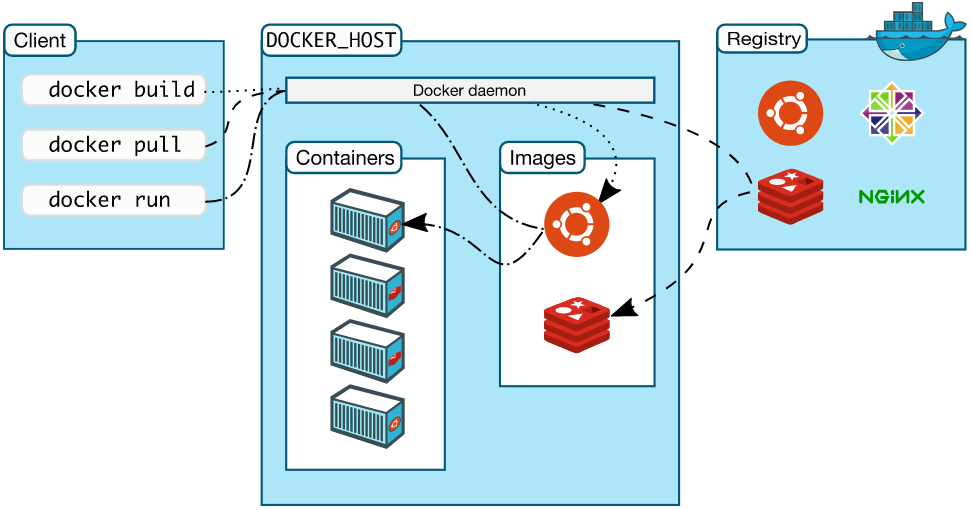
\includegraphics[width=0.8\textwidth]{Figures/docker-workflow}
    \decoRule
    \caption[Docker (Workflow)]{Flujo de trabajo en Docker \emph{\parencite{Reference20}}}
    \label{fig:docker-workflow}
\end{figure}

Como se observa en la Figura~\ref{fig:docker-workflow}, además del cliente y el demonio antes mencionados, en el despliegue y distribución de un contenedor\index{Contenedor} en Docker\index{Docker} intervienen varios elementos:

\begin{itemize}
    \item \textbf{Imágenes}: Una imagen en Docker\index{Docker} es una plantilla que detalla las instrucciones para la construcción de un contenedor\index{Contenedor}. Un usuario tiene la posibilidad de crear sus propias imágenes o utilizar las que otros usuarios hayan publicado en un registro. Para el primer caso, un usuario que quiera generar su propia imagen deberá crear un fichero \emph{Dockerfile} en el que se detallan las instrucciones (comandos) necesarias para la construcción del contenedor\index{Contenedor}.
    \item \textbf{Contenedores}: Un contenedor\index{Contenedor}, en Docker\index{Docker}, es una instancia ejecutable de una imagen. Pueden ser creados, iniciados, parados, o eliminados utilizando el cliente de Docker\index{Docker}. Se pueden conectar a una o más redes y se les puede agregar volúmenes para ampliar su espacio de almacenamiento.
    \item \textbf{Registros}: Un registro es un servidor donde los usuarios de Docker\index{Docker} pueden distribuir sus imágenes, de manera pública o privada.
\end{itemize}

%-------------------------------------------------------------------------------

\section{GitHub}

GitHub\index{GitHub} es un servicio \emph{online} que permite a los desarrolladores y a sus equipos llevar un control de versiones sobre sus proyectos \emph{software}\index{software}. Fue adquirido en 2018 por Microsoft y actualmente es la plataforma \emph{online} con mayor cantidad de repositorios de código del mundo. \emph{\parencite{Reference21}}

\begin{figure}[ht]
    \centering
    
\includegraphics[width=0.3\textwidth]{Figures/octocat}
    \decoRule
    \caption[Octocat]{Octocat (mascota de GitHub) \emph{\parencite{Reference23}}}
    \label{fig:octocat}
\end{figure}

GitHub\index{GitHub} es básicamente un SaaS de Git\index{Git}, pero con funcionalidades añadidas como la creación de \emph{issues} para el seguimiento de errores, la solicitud de cambios a código (conocidas como \emph{pull requests}), la inclusión de mecanismos automatizados (CI/CD), o la creación de \emph{wikis}, entre otros. \emph{\parencite{Reference22}}

\subsection{Dependabot}

Dependabot\index{Dependabot} es una herramienta que permite a los desarrolladores despreocuparse de actualizar las dependencias de sus proyectos \emph{software}\index{software}. Se encarga de analizar los ficheros de dependencias de un proyecto\footnote{Por ejemplo, en un proyecto Python\index{Python} estas dependencias están definidas en el fichero \emph{requirements.txt} o \emph{pyproject.toml}.} y buscar nuevas actualizaciones de estas, notificando al usuario y, en ocasiones, sugiriendo los cambios necesarios al código para su inclusión. \emph{\parencite{Reference24}}

\begin{figure}[ht]
    \centering
    
\includegraphics[width=0.2\textwidth]{Figures/dependabot-logo}
    \decoRule
    \caption[Dependabot (Logo)]{Logo de Dependabot \emph{\parencite{Reference25}}}
    \label{fig:dependabot-logo}
\end{figure}

Dependabot\index{Dependabot} fue adquirido por GitHub\index{GitHub} en 2019, lo que ha permitido una integración más estrecha con la plataforma. Mediante la creación de un fichero \emph{dependabot.yml}, los desarrolladores pueden establecer que dependencias analizar, la frecuencia de estos análisis, y la fuente desde donde se buscan actualizaciones. \emph{\parencite{Reference24}}

%% Chapter 3: Project Development

\chapter{Desarrollo del Proyecto} % Main chapter title

\label{Chapter3} % For referencing this chapter elsewhere, use \ref{Chapter3}

%-------------------------------------------------------------------------------

\section{Arquitectura del software}

El objetivo de este proyecto es proporcionar un servicio que permita analizar proyectos \emph{software}\index{software} de una manera sencilla y automatizada. Para ello, se ha llevado a cabo el desarrollo de varios \emph{sprints}, cada uno resolviendo los problemas descubiertos en el anterior:

\begin{itemize}
    \item El primer \emph{sprint} se centra en realizar un análisis de \nameref{sec:cauldron}\index{Cauldron}, una herramienta ya existente para el análisis de ecosistemas de desarrollo de \emph{software}.
    \item En el segundo \emph{sprint} se recogen las lecciones aprendidas en el anterior y se centra en el desarrollo de un primer prototipo que siente las bases de la arquitectura de la aplicación. En este prototipo, la API\index{API} consta de algunas llamadas básicas para la creación de solicitudes de análisis y el cliente es capaz de procesarlas y retornar este resultado al usuario.
    \item El tercer y último \emph{sprint} recoge el testigo del anterior y se centra en la integración de la API con \nameref{sec:grimoirelab}\index{GrimoireLab} y \nameref{sec:opensearch}\index{OpenSearch}. En este nuevo prototipo, la API\index{API} incluye nuevas estructuras y llamadas y el cliente ejecuta tareas de análisis con GrimoireLab y sube los resultados a OpenSearch para su visionado.
\end{itemize}

\subsection{Sprint 0: Etapa de análisis}

Durante la primera etapa que comprende el desarrollo de este proyecto, se ha realizado un análisis de la herramienta \nameref{sec:cauldron}\index{Cauldron}, de su proceso de desarrollo, funcionalidades y puntos de mejora, los cuales han servido como inspiración para las posteriores etapas. Se trata de una etapa de aprendizaje que sienta las bases del resto del desarrollo.

\nameref{sec:cauldron}\index{Cauldron} nace con la idea de facilitar el uso de \nameref{sec:grimoirelab}\index{GrimoireLab}, y permitir usar este a perfiles no técnicos. Es por ello que el desarrollo de este \emph{SaaS} comienza como una aplicación web, utilizando \nameref{sec:django}\index{Django} como base y Elasticsearch\index{Elasticsearch} y Kibana\index{Kibana} para el manejo de datos. \nameref{sec:cauldron}\index{Cauldron} comienza en sus inicios con pocas fuentes de datos disponibles, únicamente Git\index{Git}, aunque muy temprano comienza a incluir otras muchas como GitHub\index{GitHub}, GitLab, o Meetup, entre otras.

\nameref{sec:cauldron}\index{Cauldron} está ideado para generar informes modificables. Esto quiere decir que un usuario puede, en un momento dado, solicitar el análisis de ciertas fuentes de datos, e.g., repositorios Git\index{Git}, y una vez terminado el análisis de esta incluir una nueva fuente de datos, como Meetup. Este esquema, si bien dota a la plataforma de mayor versatilidad, acarrea varios problemas en su desarrollo y mantenimiento. Durante el desarrollo de esta característica se necesitó realizar múltiples iteraciones en los modelos de la aplicación para conseguir que solo se analizaran las nuevas fuentes de datos, y no las ya analizadas. Estas iteraciones han resultado en un esquema de modelos complejo que hace difícil su modificación.

\nameref{sec:cauldron}\index{Cauldron} hace uso de un sistema de \emph{workers} para realizar los análisis. Cada uno de estos \emph{workers} es un contenedor personalizado de \nameref{sec:grimoirelab}\index{GrimoireLab}, el cual utiliza el SDK de GrimoireLab para \nameref{sec:python}\index{Python} en la ejecución de los análisis. Estos \emph{workers} se están ejecutando continuamente, y se establece su número al comienzo del despliegue del \emph{cluster} de \emph{workers}. Las tareas de análisis que estos \emph{workers} realizan son gestionadas por un complejo componente personalizado conocido como \emph{Cauldron Pool Scheduler}, el cual realiza una asignación de recursos de análisis equitativa entre todos los usuarios de la plataforma. A pesar de los buenos resultados que este sistema genera, añade una excesiva complejidad a la asignación de tareas, lo que dificulta realizar cualquier tipo de modificación o mantenimiento a este.

\begin{figure}[ht]
    \centering
    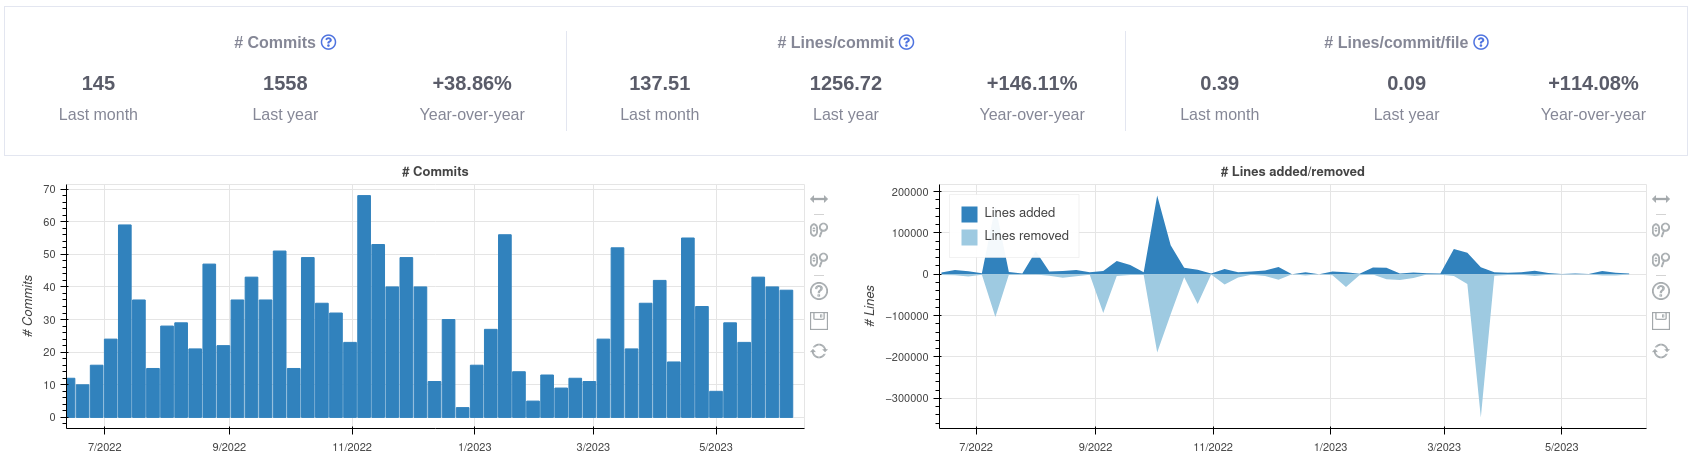
\includegraphics[width=\textwidth]{Figures/cauldron-metrics-charts}
    \decoRule
    \caption[Cauldron (Métricas)]{Métricas en Cauldron}
    \label{fig:cauldron-metrics-charts}
\end{figure}

Además de las métricas y gráficas que \nameref{sec:cauldron}\index{Cauldron} ofrece a través de Elasticsearch\index{Elasticsearch} y Kibana\index{Kibana}, existen otras muchas en la página de cada análisis (Figura~\ref{fig:cauldron-metrics-charts}). Estas están desarrolladas usando la librería \code{Bokeh} para JavaScript, la cual añade una excesiva complejidad al código al necesitar incluir grandes bloques a las plantillas de Django. Además de esto, debido a la gran cantidad de datos que algunos análisis manejan, en ocasiones la recogida de estos datos desde el \emph{cluster} de Elasticsearch\index{Elasticsearch} hace vencer un \emph{timeout} establecido, lo que provoca el fallo de la página.

Este análisis, sumado a la experiencia durante el desarrollo y mantenimiento de \nameref{sec:cauldron}\index{Cauldron} han resultado en un excelente valor didáctico, y han motivado varios de los objetivos que persigue este proyecto, los cuales serán desarrollados en los siguientes \emph{sprints}.

\subsection{Sprint 1: Grimoirebots I}

El primer prototipo de la aplicación está creado utilizando el \emph{framework} \nameref{sec:drf}\index{Django} para \nameref{sec:python}\index{Python}, y \nameref{sec:poetry}\index{Poetry} como gestor de paquetes y dependencias. Esta primera versión establece la arquitectura base de la aplicación y el esquema de comunicación entre servidor y cliente.

Para este fin, se han desarrollado los siguientes modelos\footnote{Los campos no obligatorios aparecen coloreados en gris.}:

\begin{figure}[ht]
    \centering
    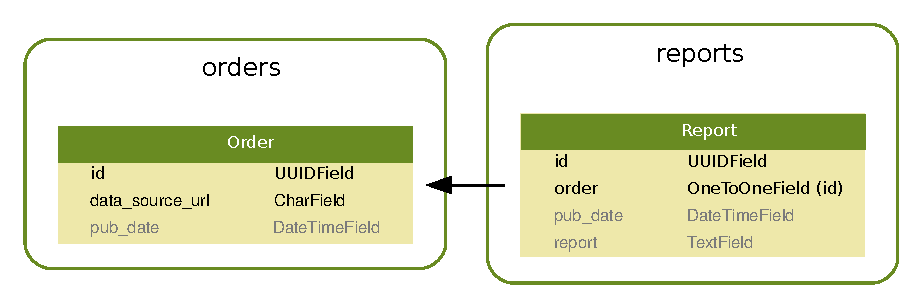
\includegraphics[width=0.8\textwidth]{Figures/grimoirebots_i_models}
    \decoRule
    \caption[Grimoirebots I (modelos)]{Modelos usados en Grimoirebots (Versión 1)}
    \label{fig:grimoirebots_i_models}
\end{figure}

\begin{itemize}
    \item \code{Order} -- Este modelo representa la solicitud hecha por un usuario. Está formado por un identificador UUID único, un \emph{string} representando la URL del repositorio git\index{Git} que se quiere analizar, y la fecha de creación de la instancia con un campo \emph{datetime}. (Figura~\ref{fig:grimoirebots_i_models})
    \item \code{Report} -- Este modelo representa el resultado de procesar una solicitud hecha por un usuario. Está formado por un identificador UUID único, una referencia a la solicitud (\code{Order}) que originó su creación, la fecha de creación de la instancia con un campo \emph{datetime}, y un \emph{string} representando el procesamiento de la solicitud. (Figura~\ref{fig:grimoirebots_i_models})
\end{itemize}

También se han desarrollado los siguientes \emph{paths} en la API\index{API}:

\begin{figure}[ht]
    \centering
    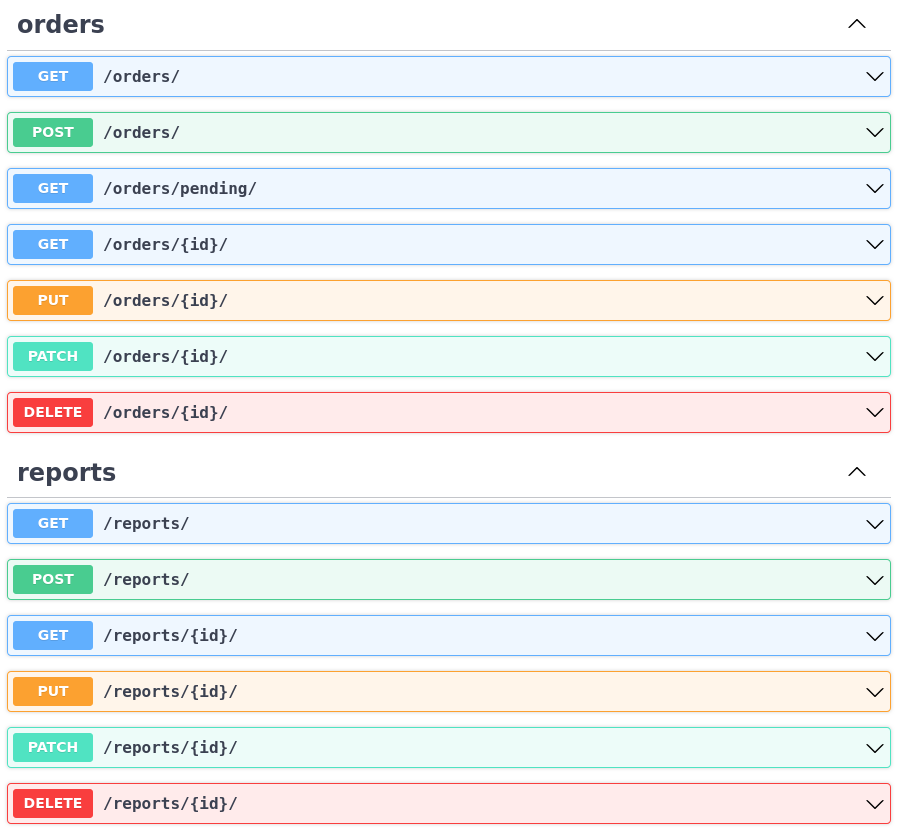
\includegraphics[width=0.8\textwidth]{Figures/grimoirebots_i_api}
    \decoRule
    \caption[Grimoirebots I (API)]{API de Grimoirebots (Versión 1)}
    \label{fig:grimoirebots_i_api}
\end{figure}

\begin{itemize}
    \item En la \emph{app} \code{orders} se han incluido \emph{paths} que permiten obtener la lista de solicitudes, la lista de solicitudes pendientes, y crear, modificar y eliminar solicitudes. (Figura~\ref{fig:grimoirebots_i_api})
    \item En la \emph{app} \code{reports} se han incluido llamadas para listar informes, y para crear, modificar y eliminar los mismos. (Figura~\ref{fig:grimoirebots_i_api})
\end{itemize}

Adicionalmente, se ha creado una imagen \nameref{sec:docker}\index{Docker} que instala las dependencias del proyecto y lo lanza utilizando \nameref{sec:gunicorn}\index{Gunicorn} como servidor WSGI, y se ha incluido el uso de \nameref{sec:dependabot}\index{Dependabot} para la comprobación de cualquier actualización en las dependencias del proyecto y avisar de esto al equipo desarrollador.

Por otra parte, en este \emph{sprint} también se ha desarrollado el cliente (o bot automático) de Grimoirebots, que es una aplicación escrita en \nameref{sec:python}\index{Python} que, haciendo uso de la librería \code{apiclient}, recoge periódicamente aquellas solicitudes pendientes de procesar y realiza un procesamiento básico de ellas. En esta parte del desarrollo aún no se había incluido \nameref{sec:grimoirelab}\index{GrimoireLab}, por lo que el procesamiento que el cliente hace de la solicitud es la construcción de un \emph{string} que contiene el identificador y el repositorio de la solicitud.

Para ilustrar el comportamiento de este prototipo, se han creado las siguientes infografías:

\begin{figure}[ht]
    \centering
    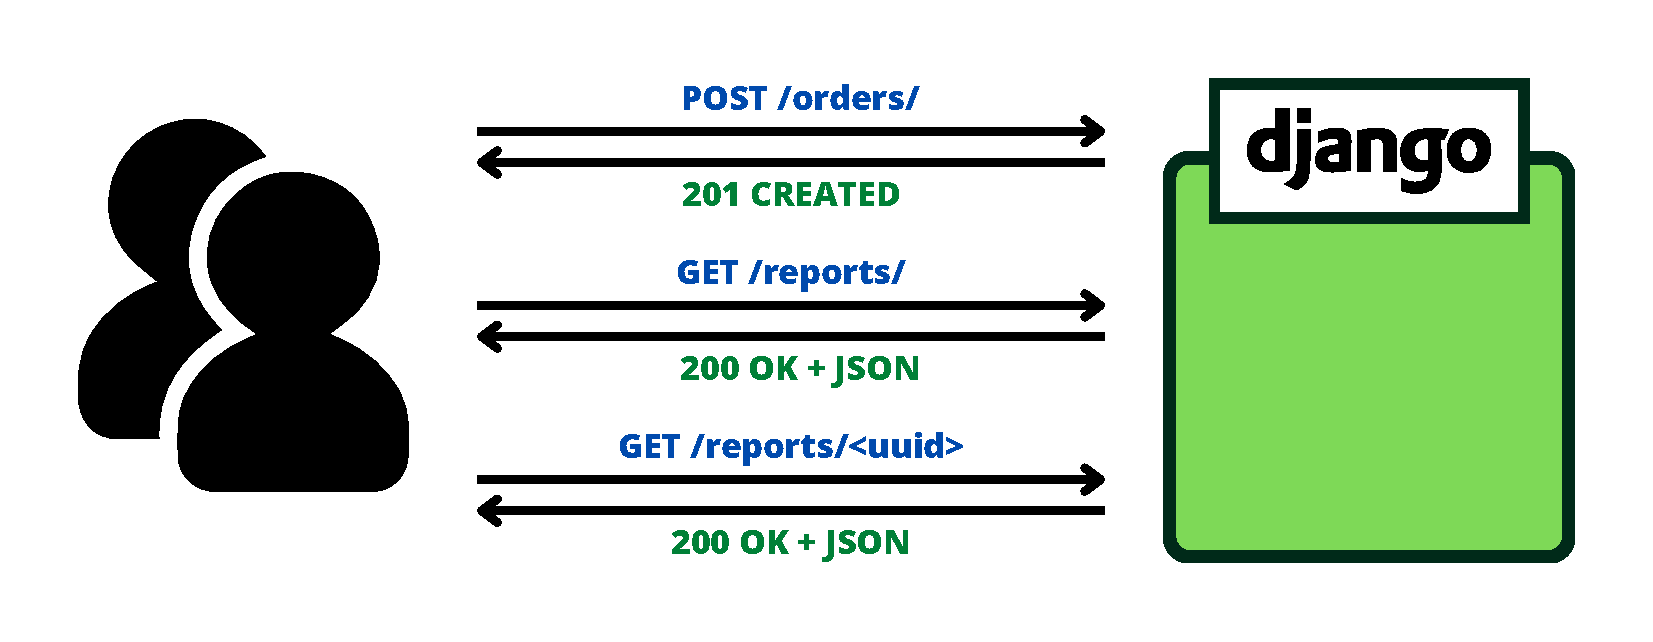
\includegraphics[width=0.8\textwidth]{Figures/grimoirebots_frontend}
    \decoRule
    \caption[Grimoirebots (\emph{Frontend})]{\emph{Frontend} de Grimoirebots (Versiones 1 y 2)}
    \label{fig:grimoirebots_frontend}
\end{figure}

Como muestra la Figura~\ref{fig:grimoirebots_frontend}, el usuario crea nuevas solicitudes de análisis realizando una llamada POST a \code{/orders/}. El usuario puede listar los informes creados mediante una llamada GET a \code{/reports/} y acceder a cada uno de ellos mediante una llamada GET a \code{/reports/<uuid>}.

\begin{figure}[ht]
    \centering
    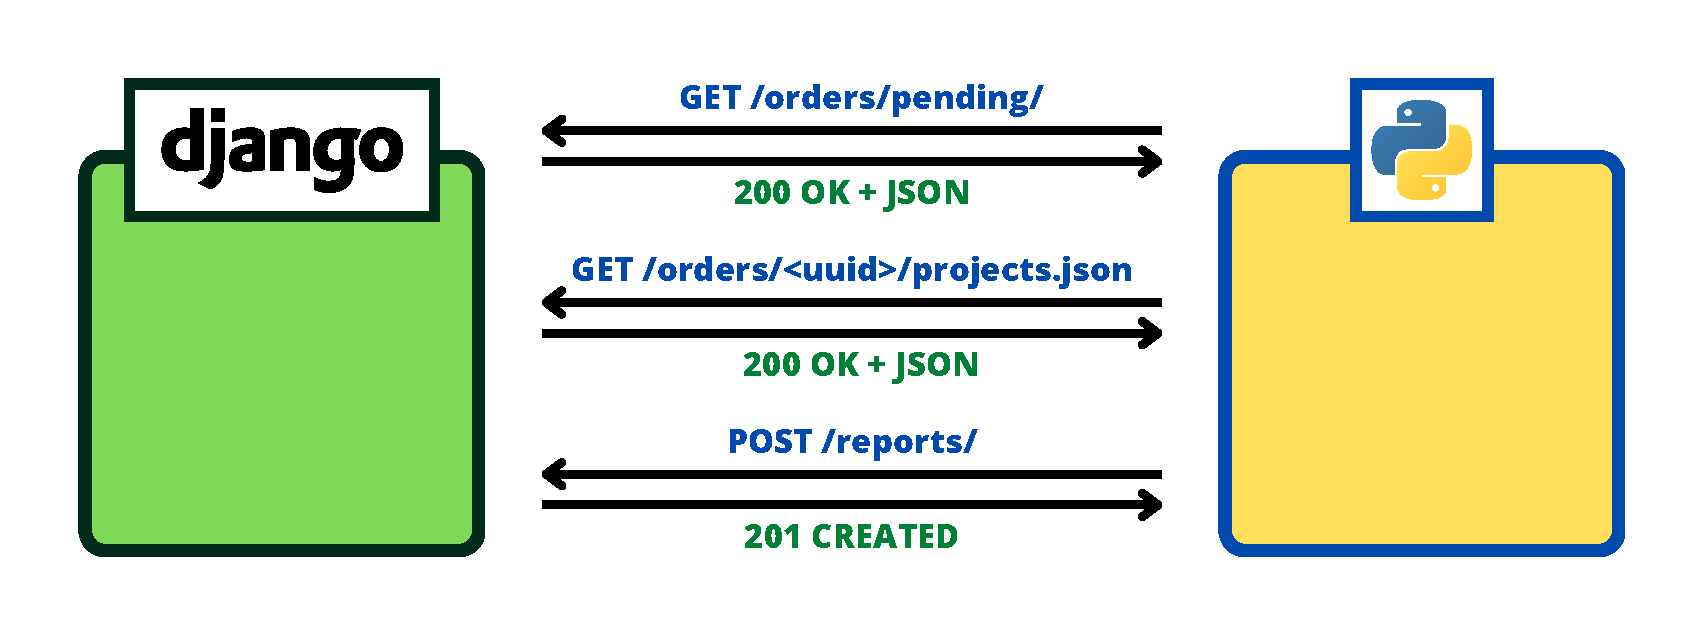
\includegraphics[width=0.8\textwidth]{Figures/grimoirebots_i_backend}
    \decoRule
    \caption[Grimoirebots I (\emph{Backend})]{\emph{Backend} de Grimoirebots (Versión 1)}
    \label{fig:grimoirebots_i_backend}
\end{figure}

Por su parte, en la Figura~\ref{fig:grimoirebots_i_backend} se incluyen las interacciones que realiza el cliente con la API\index{API} para procesar las solicitudes de los usuarios. Periódicamente, el cliente pide al servidor las solicitudes que aún no hayan sido procesadas. Por cada una de estas, pide el repositorio solicitado para analizar haciendo una llamada GET a \code{/orders/<uuid>/projects.json}. Posteriormente, realiza el procesamiento básico comentado anteriormente y realiza una llamada POST a \code{/reports/} para crear el informe y asociarlo con la solicitud del usuario.

\subsection{Sprint 2: Grimoirebots II}

Durante este \emph{sprint} se utilizan las mismas tecnologías mencionadas en el anterior, y algunas añadidas, para el desarrollo de un nuevo prototipo. Como gran aditivo, en este prototipo se incluye el uso de \nameref{sec:grimoirelab}\index{GrimoireLab} y \nameref{sec:opensearch}\index{OpenSearch} para realizar el análisis de proyectos \emph{software}\index{Software}.

Debido a esto, este prototipo actualiza los modelos de la aplicación de la siguiente forma\footnote{Igual que en el apartado anterior, los campos no obligatorios aparecen coloreados en gris.}:

\begin{figure}[ht]
    \centering
    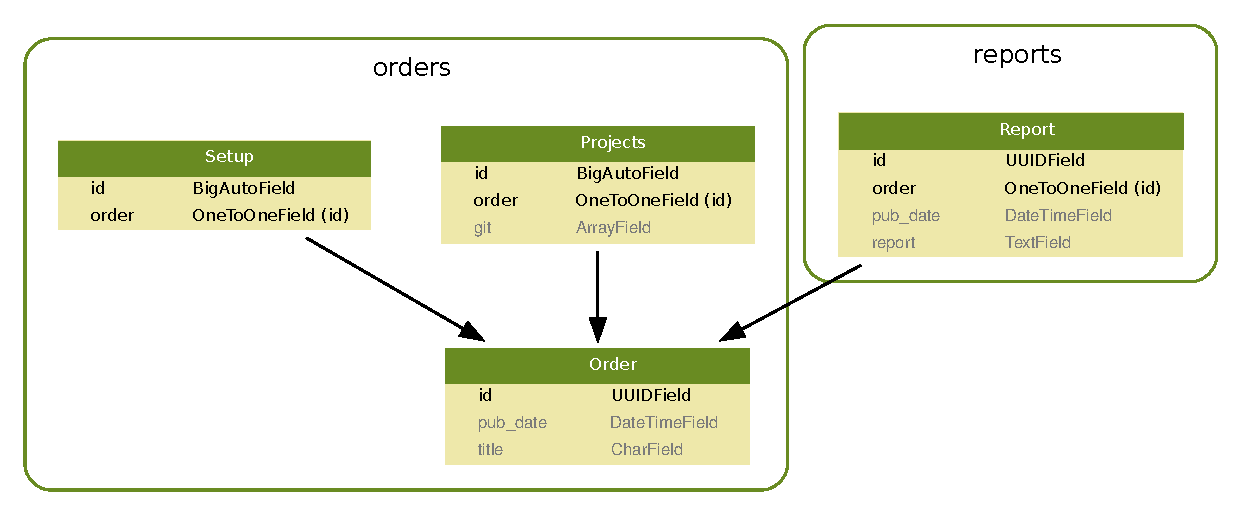
\includegraphics[width=0.8\textwidth]{Figures/grimoirebots_ii_models}
    \decoRule
    \caption[Grimoirebots II (modelos)]{Modelos usados en Grimoirebots (Versión 2)}
    \label{fig:grimoirebots_ii_models}
\end{figure}

\begin{itemize}
    \item \code{Order} -- Este modelo sigue representando la solicitud hecha por un usuario. El campo \code{data\_source\_url} ha sido eliminado y se ha incluido un campo \code{title} para que el usuario pueda identificar más fácilmente la solicitud. (Figura~\ref{fig:grimoirebots_ii_models})
    \item \code{Setup} -- Este modelo representa la configuración utilizada por \nameref{sec:grimoirelab}\index{GrimoireLab} en el análisis de proyectos \emph{software}\index{Software}. Está enlazado con una solicitud específica mediante el campo \code{order}. (Figura~\ref{fig:grimoirebots_ii_models})
    \item \code{Projects} -- Este modelo representa la lista de repositorios git\index{Git} que un usuario ha solicitado analizar. Está compuesto por un identificador numérico único, el identificador de la solicitud, y una lista de \emph{strings} con las URLs de los repositorios. (Figura~\ref{fig:grimoirebots_ii_models})
    \item \code{Report} -- Este modelo no ha sufrido cambios en este prototipo. (Figura~\ref{fig:grimoirebots_ii_models})
\end{itemize}

Los \emph{paths} que incluye la API\index{API} de este prototipo son los mismos que en el anterior, a excepción de:

\begin{figure}[ht]
    \centering
    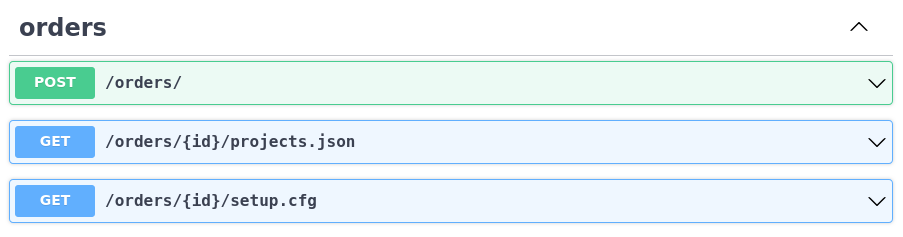
\includegraphics[width=0.8\textwidth]{Figures/grimoirebots_ii_api}
    \decoRule
    \caption[Grimoirebots II (API)]{API de Grimoirebots (Versión 2)}
    \label{fig:grimoirebots_ii_api}
\end{figure}

\begin{itemize}
    \item La llamada POST a \code{/orders/} ahora incluye los campos \code{title}, \code{projects}, y \code{setup} en el cuerpo de la petición. De esta forma, el usuario utiliza una única llamada para crear su solicitud de análisis. (Figura~\ref{fig:grimoirebots_ii_api})
    \item Se han incluido las llamadas GET para \code{/orders/<uuid>/projects.json} y para \code{/orders/<uuid>/setup.cfg} para obtener los ficheros con la lista de repositorios y la configuración para \nameref{sec:grimoirelab}\index{GrimoireLab}, respectivamente. (Figura~\ref{fig:grimoirebots_ii_api})
\end{itemize}

El cliente es modificado en este prototipo para incluir el uso de \nameref{sec:grimoirelab}\index{GrimoireLab}. La forma en que el cliente hace uso de esta herramienta es mediante un contenedor \nameref{sec:docker}\index{Docker}\footnote{\url{https://hub.docker.com/r/grimoirelab/grimoirelab}} lanzado desde el mismo cliente gracias a la librería \code{docker}.

Por otro lado, en este prototipo se incluye el uso de \nameref{sec:opensearch}\index{OpenSearch} y OpenSearch Dashboards para almacenar y visionar los datos generados por \nameref{sec:grimoirelab}\index{GrimoireLab}. Este sistema es lanzado mediante \nameref{sec:docker}\index{Docker} Compose\footnote{Docker Compose es una herramienta que permite lanzar múltiples contenedores de manera simultánea, mediante ficheros de configuración.}, y se ha construido un fichero de configuración con las características que necesita el sistema.

Igual que en el prototipo anterior, se han creado algunas infografías para ilustrar su comportamiento:

En el caso de la interacción entre usuario y servidor, el comportamiento es el mismo que en el prototipo 1. (Véase~\ref{fig:grimoirebots_frontend})

\begin{figure}[ht]
    \centering
    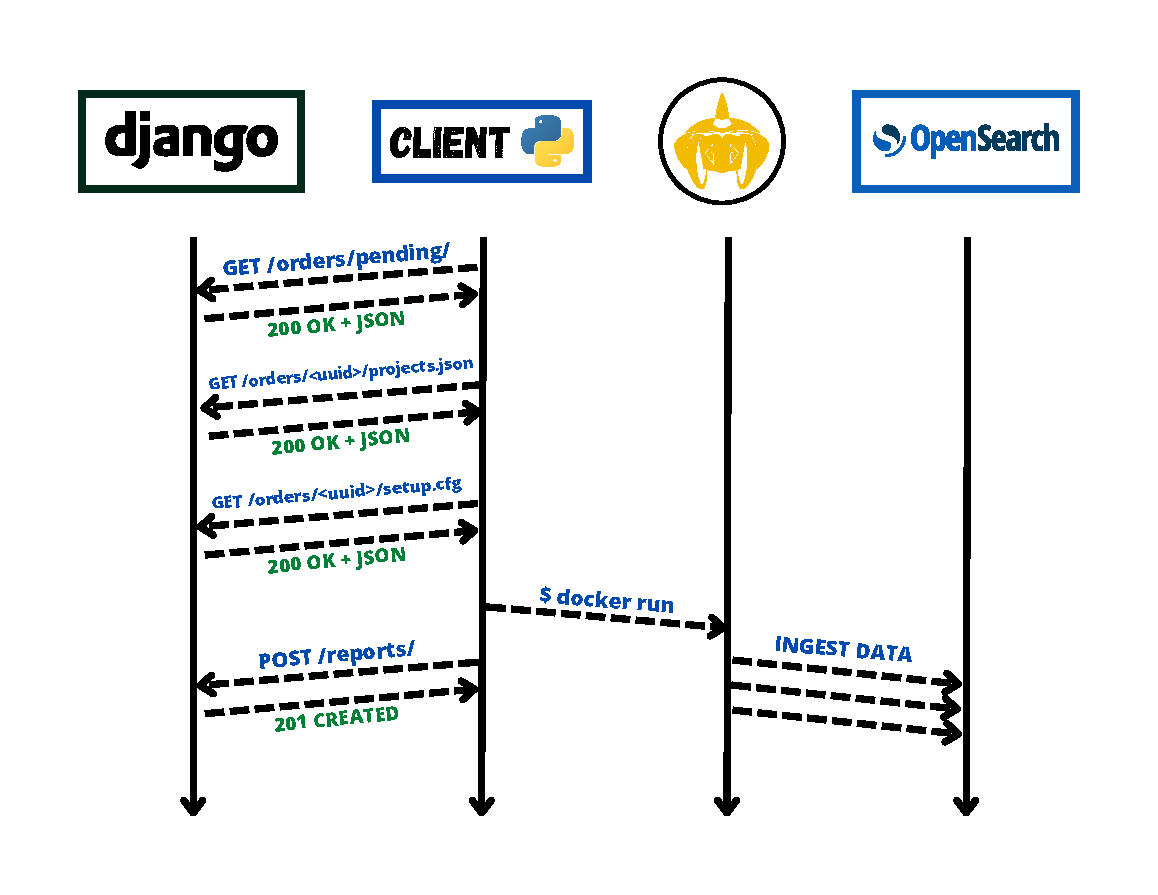
\includegraphics[width=0.8\textwidth]{Figures/grimoirebots_ii_backend}
    \decoRule
    \caption[Grimoirebots II (\emph{Backend})]{\emph{Backend} de Grimoirebots (Versión 2)}
    \label{fig:grimoirebots_ii_backend}
\end{figure}

El \emph{backend}, sin embargo, sufre varios cambios. Como muestra la Figura~\ref{fig:grimoirebots_ii_backend}, el cliente obtiene la lista de solicitudes pendientes. Para cada una de ellas obtiene los ficheros de repositorios y configuración. A continuación, utiliza la librería \code{docker} para lanzar un contenedor de \nameref{sec:grimoirelab}\index{GrimoireLab} por cada solicitud, incluyendo los ficheros antes mencionados en el volumen que utiliza cada contenedor. Por último, cada contenedor realizará el análisis de los repositorios indicados en la solicitud e ingestará los datos al \emph{cluster} de \nameref{sec:opensearch}\index{OpenSearch}, desde donde el usuario es capaz de operar con ellos.

%-------------------------------------------------------------------------------

\section{Problemas encontrados}\label{problemas-encontrados}

Durante el desarrollo del proyecto, surgieron algunas situaciones que dificultaron la finalización del mismo.

Se quiso utilizar, al comienzo, la versión estándar de \nameref{sec:django}\index{Django} incluyendo su sistema de \emph{templates}. Esto era debido a que la aplicación contaba en un principio con un \emph{frontend} con interfaz gráfica, la cual sería accesible desde un navegador web. Debido a las ventajas que suponía el uso de \nameref{sec:drf} (como el uso de \emph{serializers}) se decidió utilizar este para parte del \emph{backend}. Sin embargo, este módulo funcionaba de manera bastante mala con el sistema de \emph{templates} de \nameref{sec:django}. Finalmente, se decidió continuar usando \nameref{sec:drf} y dejar de lado la interfaz gráfica, debido a la gran ventaja que suponía el primero frente al segundo.

Uno de los ficheros que \nameref{sec:grimoirelab}\index{GrimoireLab} utiliza, el llamado fichero de configuración, utiliza un formato con una estructura muy similar al que puede encontrarse en los ficheros INI usados en Microsoft Windows. Este formato no es soportado de forma nativa por \nameref{sec:drf}, y causó varios retrasos tratando de implementar una solución para hacerlo viable. Finalmente se decidió hacer que la API\index{API} devolviera el fichero con formato JSON\index{JSON} y luego, en el cliente, convertir este al formato necesario usando la librería \code{configparser}. Esto fue posible debido a que ambos formatos comparten similitudes que hacen viable su conversión.

Durante la última etapa del desarrollo, se quiso realizar una implementación de Grimoirebots desarrollada con \nameref{sec:fastapi}\index{FastAPI}, con el fin de comparar este con \nameref{sec:drf}. Sin embargo, este prototipo nunca llegó a ver la luz por complicaciones en su desarrollo, aunque se realizaron algunas pruebas que pueden encontrarse en \nameref{sec:github}\index{GitHub}\footnote{\url{https://github.com/merinhunter/grimoirebots-fastapi}}.

Además de todo lo anterior, existieron otros pequeños problemas que ralentizaron el desarrollo del proyecto, como la complejidad de ejecutar contenedores\index{Contenedor} desde otro contenedor, o la falta de documentación en algunos módulos de \nameref{sec:grimoirelab}. Sin embargo, todos estos incidentes tienen un alto valor didáctico, y su documentación permitirá no volver a cometerlos en el futuro.

%-------------------------------------------------------------------------------

\section{Tiempo dedicado}

El desarrollo de cada \emph{sprint} ha requerido un tiempo de trabajo distinto, dedicado a diferentes actividades. En esta sección se detalla el tiempo invertido en cada etapa:

\begin{itemize}
    \item El primer \emph{sprint}, al tratarse de una etapa de aprendizaje, se ha centrado exclusivamente en la investigación. Debido a que ya se contaba con un conocimiento inicial sobre la herramienta analizada, no ha supuesto un número excesivo de horas, finalizando este sprint a las tres semanas de iniciar el proyecto. Con una media diaria de dos horas, esta etapa ha supuesto un total de \textbf{42 horas}.
    \item El segundo \emph{sprint} marca el comienzo del desarrollo del primer prototipo. Aunque principalmente se ha dedicado tiempo a la creación de componentes software, también se ha dedicado una pequeña parte del tiempo al estudio de diferentes herramientas que pudieran ayudar al desarrollo del prototipo. En total, la finalización de esta etapa ha supuesto dos semanas de investigación y cuatro de desarrollo, con una media de dos horas diarias, haciendo un total de \textbf{84 horas}.
    \item El tercer \emph{sprint}, al partir de la base desarrollada en el sprint anterior, no debería haber requerido demasiado tiempo de trabajo. Sin embargo, los problemas que se detallan en el Capítulo~{\ref{problemas-encontrados}}, han incrementado el tiempo dedicado a esta etapa. Esta fase ha requerido utilizar dos semanas para investigación sobre cómo realizar la integración de GrimoireLab y OpenSearch con el proyecto, y cinco semanas de desarrollo para su implementación. Con una media diaria de dos horas, esta etapa se ha finalizado en \textbf{98 horas}.
\end{itemize}

En total, la finalización del proyecto ha requerido aproximadamente \textbf{224 horas} de trabajo, con mayor tiempo dedicado al desarrollo.

%% Chapter 4: System Specifications

\chapter{Especificaciones del sistema} % Main chapter title

\label{Chapter4} % For referencing this chapter elsewhere, use \ref{Chapter4}

%-------------------------------------------------------------------------------

\section{Requisitos}

En esta sección se describen todas las herramientas y \emph{software}\index{Software} que es necesario instalar en el sistema antes de la ejecución de Grimoirebots.

\begin{itemize}
    \item \textbf{Docker}\index{Docker} -- La ejecución de Grimoirebots se realiza usando contenedores Docker, por lo que su instalación es obligatoria. La instalación de Docker es diferente en función del Sistema Operativo utilizado, encontrándose una guía para los más utilizados en su página de documentación\footnote{\url{https://docs.docker.com/get-docker/}}.
    \item \textbf{Docker Compose} -- La herramienta Docker Compose permite ejecutar varios contenedores\index{Contenedor} al mismo tiempo, gracias a ficheros de configuración. Su instalación es necesaria para la ejecución del \emph{cluster} de OpenSearch\index{OpenSearch} y de la base de datos PostgreSQL\index{PostgreSQL}. De nuevo, su instalación varía en función del Sistema Operativo, encontrándose una guía de instalación en su página de documentación\footnote{\url{https://docs.docker.com/compose/install/}}.
\end{itemize}

Al tratarse de una aplicación \emph{dockerizada}, todos los demás requisitos están incluidos en los contenedores\index{Contenedor}. A pesar de no ser necesaria su instalación, y simplemente para dar a conocerlos, estos son:

\begin{itemize}
    \item \textbf{Python}\index{Python} -- Para la ejecución tanto del servidor como del cliente se ha utilizado \code{Python 3.11}.
    \item \textbf{Poetry}\index{Poetry} -- La gestión (e instalación) de paquetes en Grimoirebots se realiza con la versión más actualizada de esta herramienta.
    \item \textbf{Dependencias de los proyectos Python} -- Esto incluye las últimas versiones disponibles de las librerías \code{Django}, \code{gunicorn}\index{Gunicorn}, \code{djangorestframework}, \code{psycopg}, \code{pyyaml}, \code{uritemplate}, \code{api-client} y \code{configparser}.
    \item \textbf{PostgreSQL}\index{PostgreSQL} -- La base de datos SQL que utiliza Django\index{Django}. La versión que utiliza el proyecto es la 15.1.
    \item \textbf{OpenSearch}\index{OpenSearch} -- Se utiliza para almacenar los resultados de los análisis con GrimoireLab\index{GrimoireLab}. La versión que utiliza el proyecto es la versión más actualizada de la versión 1\footnote{GrimoireLab no soporta versiones superiores a la 2, por lo que el proyecto está limitado por esta parte.}.
    \item \textbf{OpenSearch Dashboards} -- Se utiliza la misma versión que para OpenSearch.
\end{itemize}

\section{Configuración}

Antes de realizar el despliegue de la aplicación y sus componentes, es necesario configurar estos. En esta sección se detallan los pasos necesarios para preparar un entorno local para el despliegue de Grimoirebots\footnote{Se asume que el despligue se realizará en una máquina Linux local.}.

Primero, es necesario descargar o clonar el repositorio de Grimoirebots:

\begin{lstlisting}[language=bash]
$ git clone https://github.com/merinhunter/grimoirebots.git
\end{lstlisting}

A continuación, se debe construir la imagen Docker\index{Docker}:

\begin{lstlisting}[language=bash]
$ cd grimoirebots/
$ docker build -t grimoirebots .
\end{lstlisting}

Una vez hecho esto, es necesario descargar o clonar el repositorio con los ficheros de configuración para desplegar Grimoirebots con Docker Compose:

\begin{lstlisting}[language=bash]
$ git clone https://github.com/merinhunter/grimoirebots-deployment.git
\end{lstlisting}

En este repositorio es posible encontrar ficheros YAML con la configuración para desplegar tanto la base de datos PostgreSQL\index{PostgreSQL} como el servidor Django\index{Django}.

Los ficheros de configuración están preparados para funcionar una vez descargados, pero es recomendable modificar las claves por defecto en los siguientes ficheros:

\begin{lstlisting}[language=bash]
$ cd grimoirebots-deployment/
$ vim grimoirebots/docker-compose.yml
$ vim postgresql/docker-compose.yml
\end{lstlisting}

Las variables que se debe modificar son \code{DJANGO\_SECRET\_KEY} y \code{DATABASE\_PASSWORD}\footnote{Esta variable aparece dos veces en el fichero \code{grimoirebots/docker-compose.yml}.}.

A continuación, es necesario descargar o clonar el repositorio del cliente de Grimoirebots:

\begin{lstlisting}[language=bash]
$ git clone https://github.com/merinhunter/grimoirebots-client.git
\end{lstlisting}

E igual que en pasos anteriores, construir la imagen Docker\index{Docker}:

\begin{lstlisting}[language=bash]
$ cd grimoirebots-client/
$ docker build -t grimoirebots-client .
\end{lstlisting}

Por último, el \emph{cluster} de OpenSearch\index{OpenSearch} requiere que, en el \emph{host}, el valor de la variable \code{vm.max\_map\_count} sea de, al menos, 262144:

\begin{lstlisting}[language=bash]
$ sudo vim /etc/sysctl.conf

# Include the following line at the end of the file
vm.max_map_count=262144

$ sudo sysctl -p
\end{lstlisting}

\section{Despliegue}

Una vez realizada la correcta configuración de todos los componentes, es posible llevar a cabo su despliegue. En esta sección se detallan todos los pasos necesarios para poner Grimoirebots en funcionamiento.

El primer paso es poner en marcha el \emph{cluster} de OpenSearch\index{}:

\begin{lstlisting}[language=bash]
$ cd grimoirebots-deployment/opensearch/
$ docker compose up -d
\end{lstlisting}

A continuación, se despliega la base de datos PostgreSQL\index{}:

\begin{lstlisting}[language=bash]
$ cd grimoirebots-deployment/postgresql/
$ docker compose up -d
\end{lstlisting}

Se continúa con el despliegue del cliente de Grimoirebots:

\begin{lstlisting}[language=bash]
$ cd grimoirebots-deployment/grimoirebots-client/
$ docker compose up -d
\end{lstlisting}

Y, finalmente, se despliega el servidor de Grimoirebots:

\begin{lstlisting}[language=bash]
$ cd grimoirebots-deployment/grimoirebots/
$ docker compose up -d
\end{lstlisting}

En este punto, Grimoirebots debería estar escuchando peticiones en el \emph{endpoint}\\\code{http://localhost:8000}, y debería ser posible acceder a OpenSearch Dashboards en el \emph{endpoint} \code{http://localhost:5601}.

Para comprobarlo, es posible realizar una petición al servidor a través de la terminal:

\begin{lstlisting}[language=bash]
$ curl http://localhost:8000
openapi: 3.0.2
info:
  title: Grimoirebots
  version: 0.1.0
  description: Run GrimoireLab in the cloud!
...
\end{lstlisting}

Accediendo a la dirección \code{http://localhost:5601} usando un navegador web, se debería ver la página de \emph{login} de OpenSearch Dashboards tal como aparece en la Figura~\ref{fig:opensearch-dashboards-login}.

\begin{figure}[ht]
    \centering
    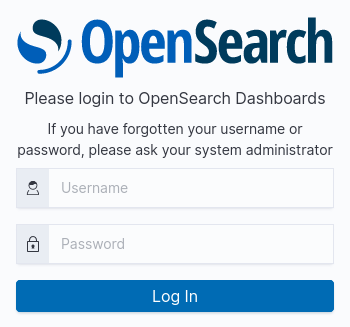
\includegraphics[width=0.4\textwidth]{Figures/opensearch-dashboards-login}
    \decoRule
    \caption[OpenSearch Dashboards (\emph{Login})]{Página de \emph{login} en OpenSearch Dashboards}
    \label{fig:opensearch-dashboards-login}
\end{figure}

\section{Ejemplo de uso}

Para ilustrar el funcionamiento de Grimoirebots, en esta sección se va a mostrar un caso de uso en el que un usuario quiere analizar una serie de repositorios git\index{Git}, y después visualizar los datos generados en este análisis.

Para ello se va a hacer uso de la herramienta \nameref{sec:postman}\index{Postman}, que permite realizar fácilmente peticiones HTTP\index{HTTP} a diferentes \emph{endpoints}.

\subsection{Creación de una petición de análisis}

El primer paso será realizar una petición POST al \emph{endpoint} \code{http://localhost:8000/\\orders/}, con la configuración del análisis en el campo \emph{body} de la solicitud (Figura~\ref{fig:example1}).

\begin{figure}[ht]
    \centering
    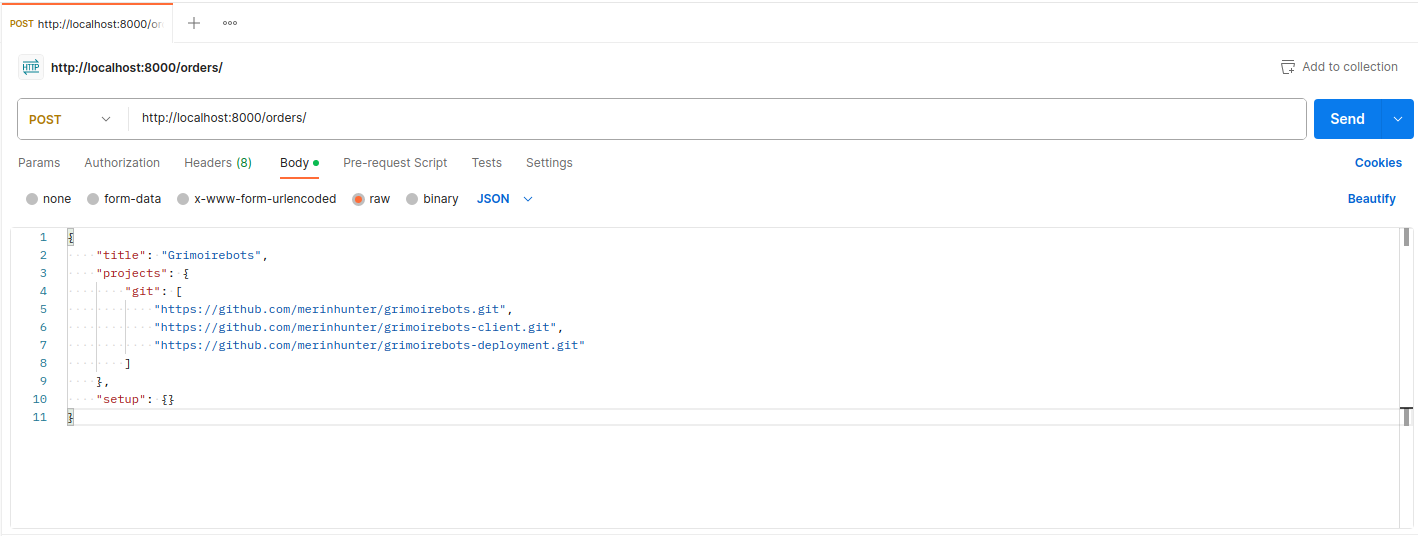
\includegraphics[width=\textwidth]{Figures/example1}
    \decoRule
    \caption[Grimoirebots (Creación de análisis)]{Creación de una solicitud de análisis en Grimoirebots}
    \label{fig:example1}
\end{figure}

La solicitud dará como respuesta un \textbf{201 Created} (Figura~\ref{fig:example2}).

\begin{figure}[ht]
    \centering
    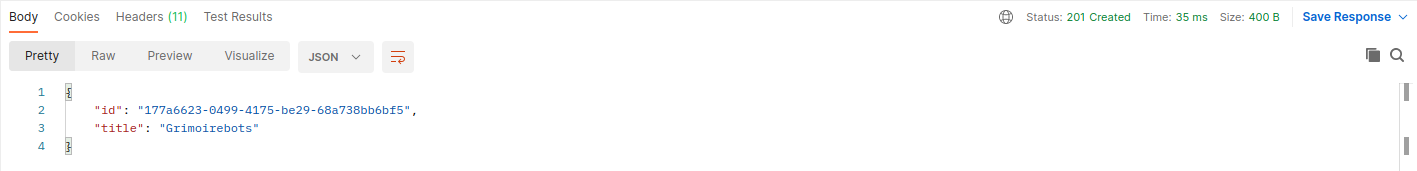
\includegraphics[width=\textwidth]{Figures/example2}
    \decoRule
    \caption[Grimoirebots (Respuesta de creación de análisis)]{Respuestas a la creación de una solicitud de análisis en Grimoirebots}
    \label{fig:example2}
\end{figure}

Si se realiza una petición GET al \emph{endpoint} \code{http://localhost:8000/orders/\\<order\_id>}, sustituyendo \code{<order\_id>} por el identificador de la solicitud de análisis enviada, se puede obtener el objeto creado (Figura~\ref{fig:example3}).

\begin{figure}[ht]
    \centering
    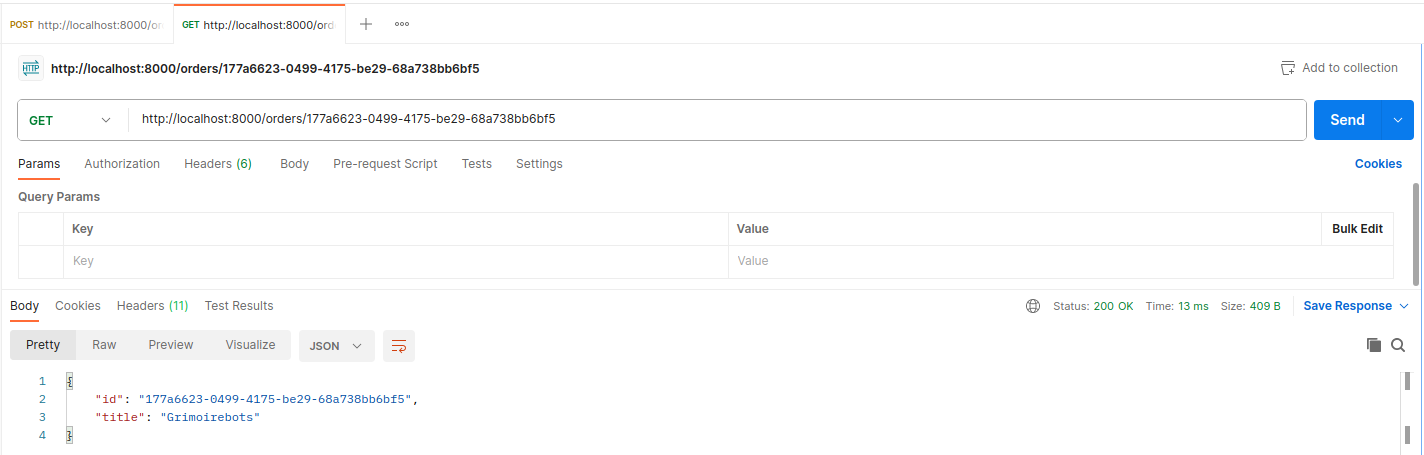
\includegraphics[width=\textwidth]{Figures/example3}
    \decoRule
    \caption[Grimoirebots (Solicitud de análisis)]{Solicitud de análisis en Grimoirebots}
    \label{fig:example3}
\end{figure}

Y realizando una petición GET a los \emph{endpoints} \code{http://localhost:8000/orders/\\<order\_id>/projects.json} y \code{http://localhost:8000/orders/<order\_id>/\\setup.cfg} se pueden obtener los ficheros de configuración de \nameref{sec:grimoirelab}\index{GrimoireLab} para el análisis (Figura~\ref{fig:example4} y Figura~\ref{fig:example5}).

\begin{figure}[ht]
    \centering
    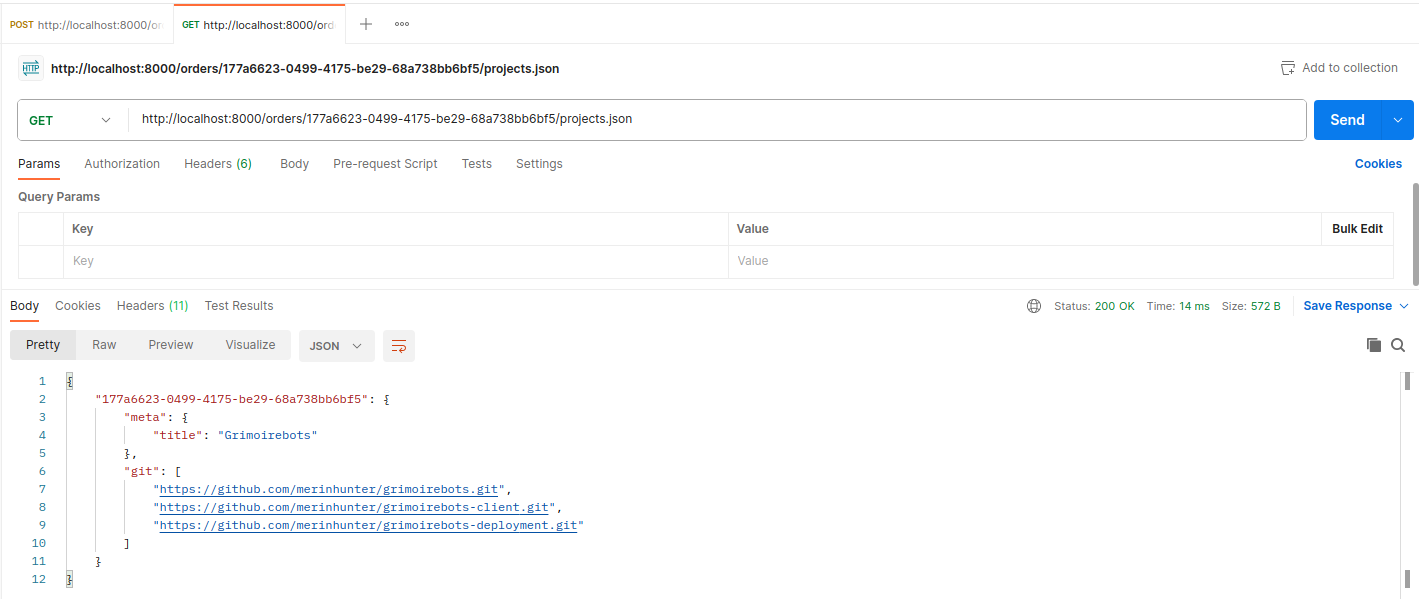
\includegraphics[width=\textwidth]{Figures/example4}
    \decoRule
    \caption[Análisis en Grimoirebots (Fichero de repositorios)]{Fichero de repositorios de un análisis en Grimoirebots}
    \label{fig:example4}
\end{figure}

\begin{figure}[ht]
    \centering
    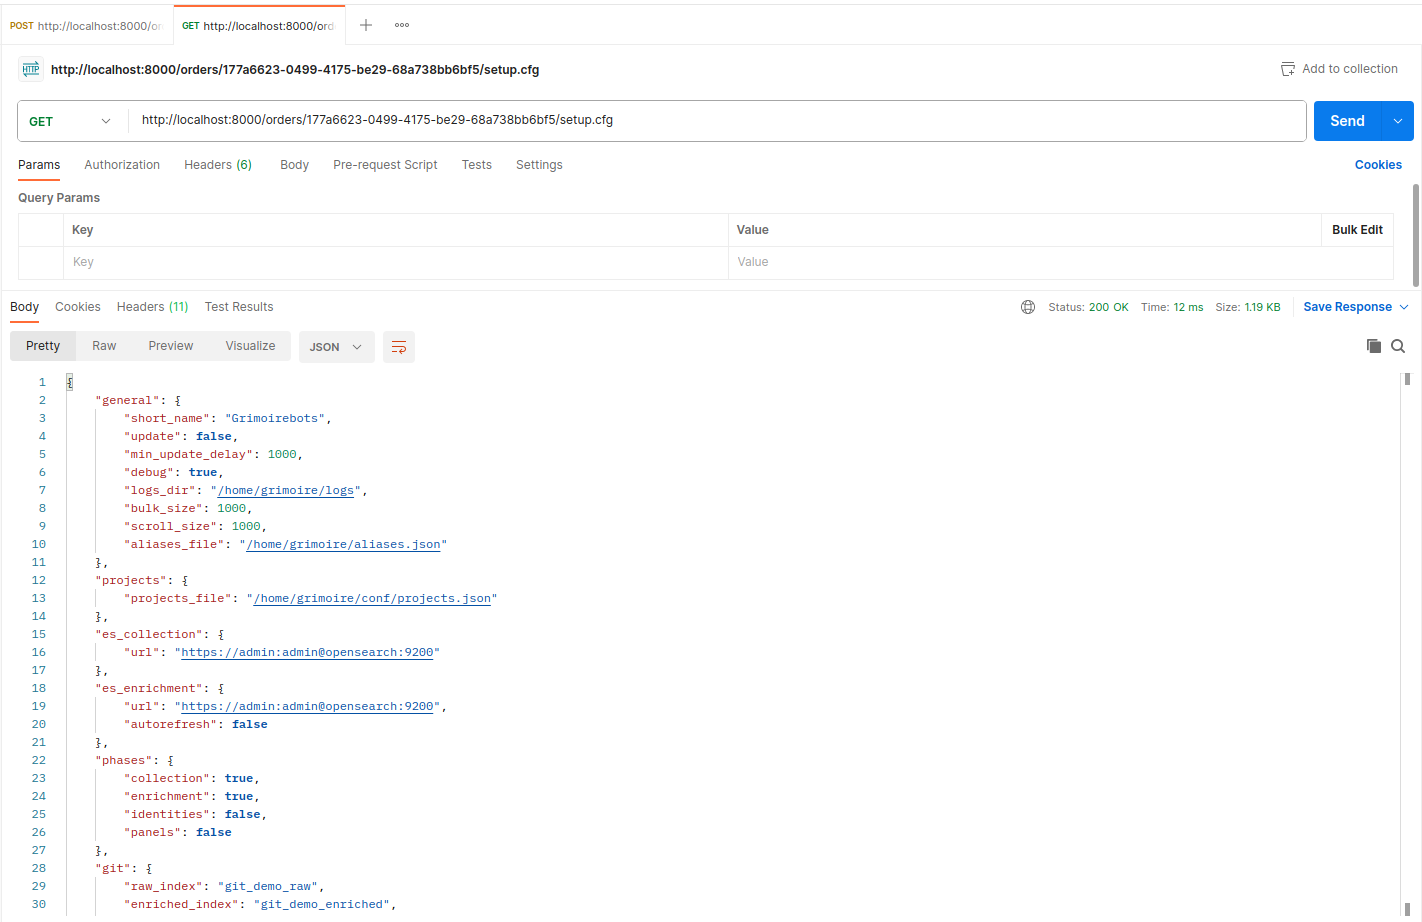
\includegraphics[width=\textwidth]{Figures/example5}
    \decoRule
    \caption[Análisis en Grimoirebots (Fichero de configuración)]{Fichero de configuración de un análisis en Grimoirebots}
    \label{fig:example5}
\end{figure}

A continuación, el cliente de Grimoirebots solicitará al servidor estos ficheros. Se pueden comprobar los logs del contenedor para asegurarnos de ello:

\begin{lstlisting}[language=bash]
$ docker logs grimoirebots-client
2023-06-18 17:00:54,511 - INFO - Retrieving pending orders from http://localhost:8000
2023-06-18 17:00:54,523 - INFO - Retrieved 1 orders
2023-06-18 17:00:54,523 - INFO - Processing order 177a6623-0499-4175-be29-68a738bb6bf5
2023-06-18 17:00:54,523 - INFO - Retrieving projects.json for order 177a6623-0499-4175-be29-68a738bb6bf5
2023-06-18 17:00:54,536 - INFO - File projects.json for order 177a6623-0499-4175-be29-68a738bb6bf5 saved at reports/177a6623-0499-4175-be29-68a738bb6bf5/projects.json
2023-06-18 17:00:54,536 - INFO - Retrieving setup.cfg for order 177a6623-0499-4175-be29-68a738bb6bf5
2023-06-18 17:00:54,550 - INFO - File setup.cfg for order 177a6623-0499-4175-be29-68a738bb6bf5 saved at reports/177a6623-0499-4175-be29-68a738bb6bf5/setup.cfg
2023-06-18 17:00:54,550 - INFO - Starting GrimoireLab container
2023-06-18 17:00:54,676 - INFO - Analysis for 177a6623-0499-4175-be29-68a738bb6bf5 has finished
2023-06-18 17:00:54,676 - INFO - Creating report for order 177a6623-0499-4175-be29-68a738bb6bf5
2023-06-18 17:00:54,690 - INFO - Report 9ddf60a6-964f-41d5-9493-f058cbdc2c41 created for order 177a6623-0499-4175-be29-68a738bb6bf5
\end{lstlisting}

Y una vez que el cliente haya comenzado el análisis, se puede realizar una petición GET al \emph{endpoint} \code{http://localhost:8000/reports/} para comprobar que existe un informe asociado a la petición inicial (Figura~\ref{fig:example6}).

\begin{figure}[ht]
    \centering
    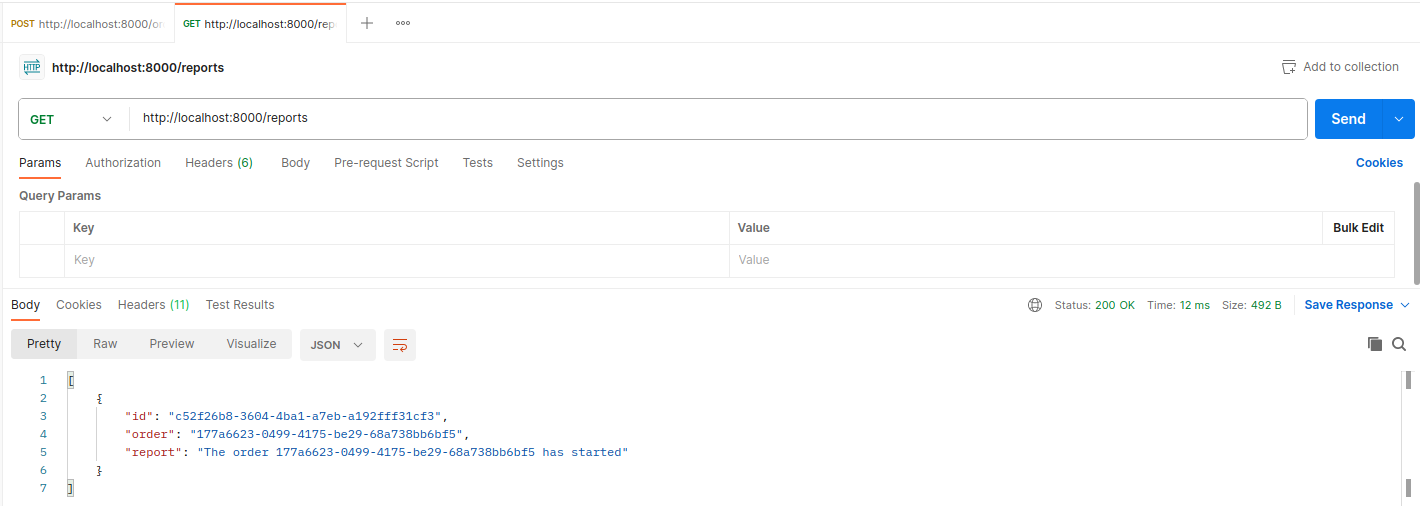
\includegraphics[width=\textwidth]{Figures/example6}
    \decoRule
    \caption[Grimoirebots (Informe)]{Informe en Grimoirebots}
    \label{fig:example6}
\end{figure}

A partir de este momento, el análisis se está llevando a cabo en un contenedor de \nameref{sec:grimoirelab}\index{GrimoireLab}. El seguimiento de este análisis se puede realizar revisando en tiempo real los logs del contenedor, necesitando localizar a este primero:

\begin{lstlisting}[language=bash]
$ docker ps
CONTAINER ID   IMAGE    ...    NAMES
b0a1f6acf822   grimoirelab/grimoirelab:0.10.0 ... grimoirelab-177a6623-0499-4175-be29-68a738bb6bf5
...

$ docker logs -f grimoirelab-177a6623-0499-4175-be29-68a738bb6bf5
2023-06-18 17:00:55,882 - sirmordred.sirmordred - INFO -
2023-06-18 17:00:55,882 - sirmordred.sirmordred - INFO - ----------------------------
2023-06-18 17:00:55,882 - sirmordred.sirmordred - INFO - Starting SirMordred engine ...
2023-06-18 17:00:55,882 - sirmordred.sirmordred - INFO - ----------------------------
2023-06-18 17:00:55,885 - urllib3.connectionpool - DEBUG - Starting new HTTPS connection (1): localhost:9200
...
\end{lstlisting}

\subsection{Visualización de datos en OpenSearch}

Una vez que el análisis con \nameref{sec:grimoirelab}\index{GrimoireLab} haya concluido, es posible visualizar los datos del análisis y construir gráficos y métricas con ellos accediendo a \nameref{sec:opensearch}\index{OpenSearch} Dashboards. Este servicio debería estar disponible navegando a la dirección \code{http://\\localhost:5601} con un navegador web.

Las credenciales por defecto son \textbf{admin} para el usuario y la contraseña. Al acceder, lo primero que se pedirá es seleccionar el \emph{tenant} de trabajo. Para el ejemplo se seleccionará el \emph{tenant} global (Figura~\ref{fig:opensearch-tenant}).

\begin{figure}[ht]
    \centering
    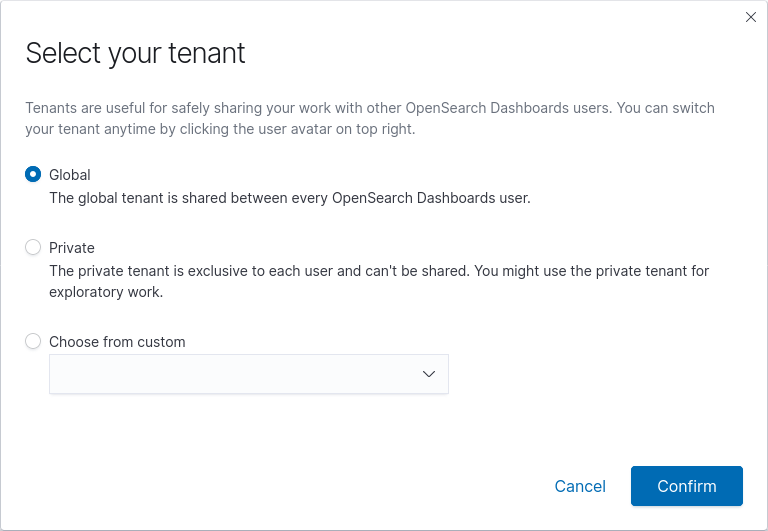
\includegraphics[width=\textwidth]{Figures/opensearch-tenant.png}
    \decoRule
    \caption[OpenSearch (Selección de \emph{tenant})]{Selección de \emph{tenant} en OpenSearch}
    \label{fig:opensearch-tenant}
\end{figure}

Si se accede a la sección \code{Index Management / Indices} es posible comprobar que existen algunos índices originados por \nameref{sec:grimoirelab}\index{GrimoireLab}, como \code{git\_demo\_raw} o \code{git\_demo\_\\enriched} (Figura~\ref{fig:opensearch-indices}).

\begin{figure}[ht]
    \centering
    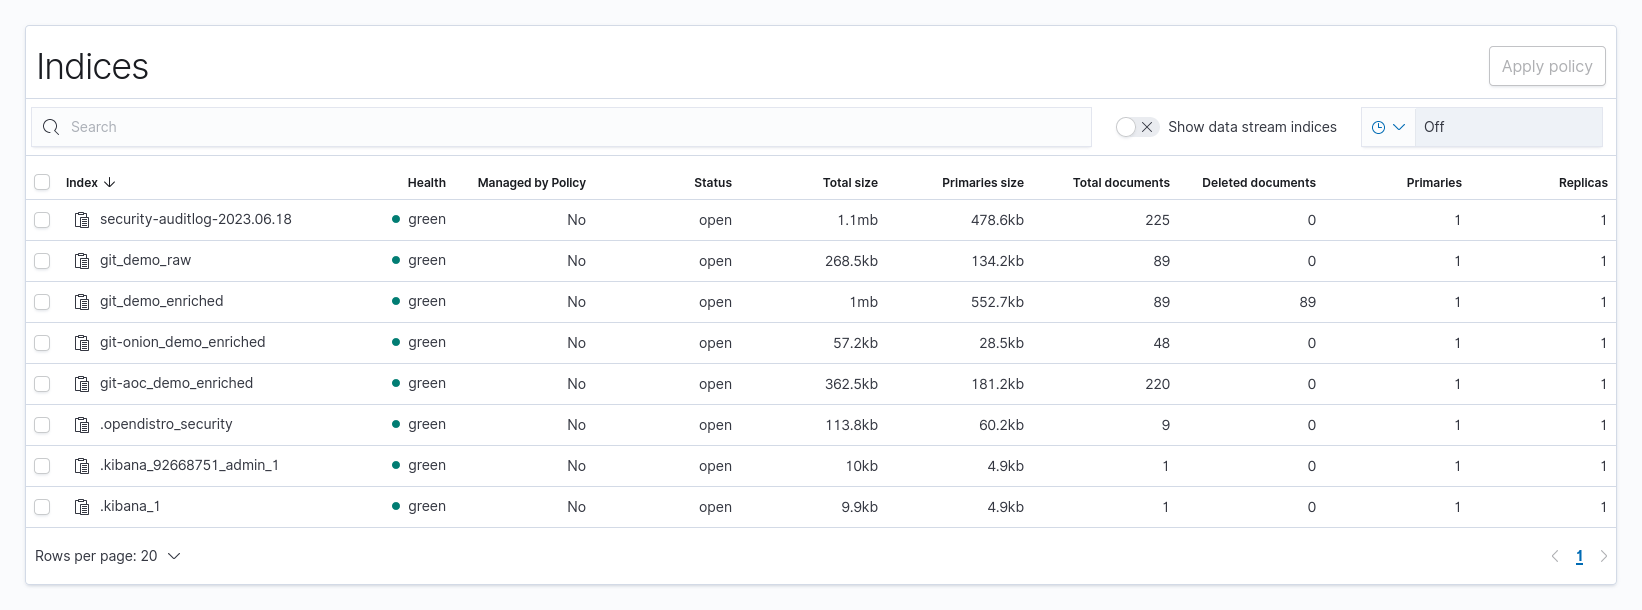
\includegraphics[width=\textwidth]{Figures/opensearch-indices.png}
    \decoRule
    \caption[OpenSearch (Índices)]{Índices en OpenSearch}
    \label{fig:opensearch-indices}
\end{figure}

Para visualizar los datos, es necesario primero crear un \emph{index pattern}. Esto sirve para que \nameref{sec:opensearch}\index{OpenSearch} sepa qué campos de los documentos debe utilizar en la indexación de la información. Para ello, se debe hacer clic en la pestaña \emph{Discover}, en la barra lateral, desde donde se solicitará la creación de un \emph{index pattern}. Para este ejemplo se utilizará como \emph{index pattern} el valor \code{git}, que concuerda con uno de los índices existentes (Figura~\ref{fig:opensearch-index-pattern-creation}).

\begin{figure}[ht]
    \centering
    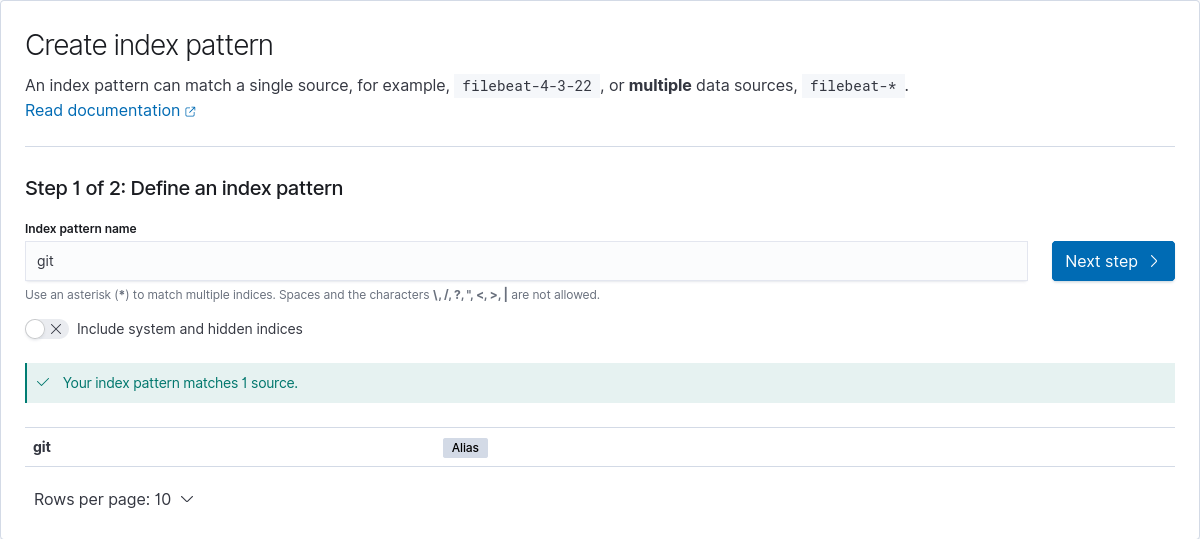
\includegraphics[width=\textwidth]{Figures/opensearch-index-pattern-creation.png}
    \decoRule
    \caption[OpenSearch (Creación de \emph{Index Pattern})]{Creación de \emph{Index Pattern} en OpenSearch}
    \label{fig:opensearch-index-pattern-creation}
\end{figure}

Como campo temporal se utilizará el campo \code{utc\_commit}, que corresponde con la hora UTC en la que cada \emph{commit} se realizó (Figura~\ref{fig:opensearch-index-pattern-timestamp}).

\begin{figure}[ht]
    \centering
    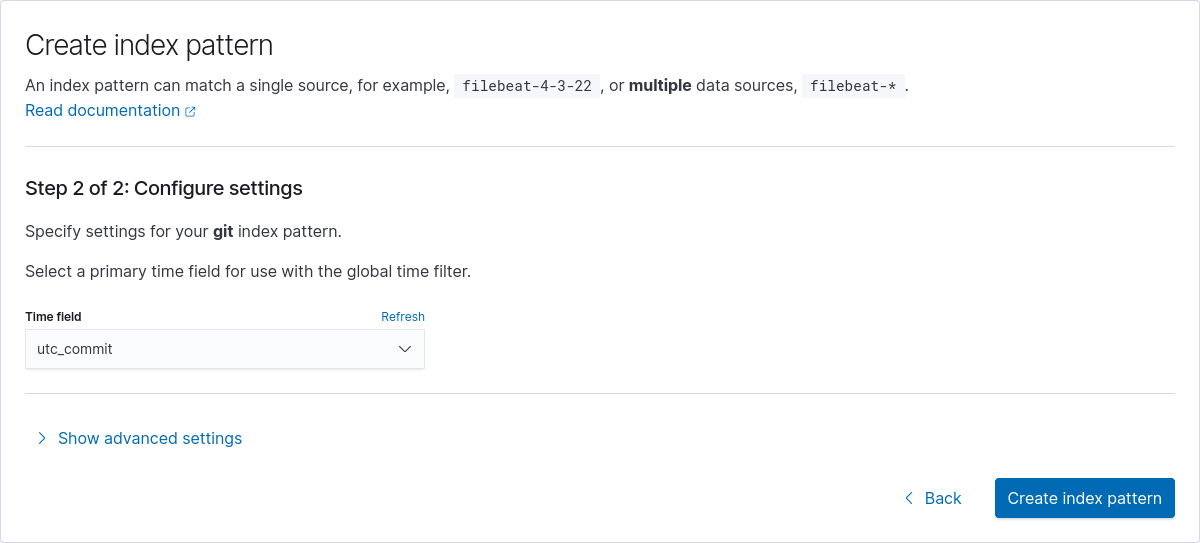
\includegraphics[width=\textwidth]{Figures/opensearch-index-pattern-timestamp.png}
    \decoRule
    \caption[OpenSearch (Creación de \emph{Index Pattern}) Cont.]{Creación de \emph{Index Pattern} en OpenSearch (Cont.)}
    \label{fig:opensearch-index-pattern-timestamp}
\end{figure}

Una vez creado el \emph{index pattern}, es posible hacer clic en \emph{Discover} y visualizaer algunos de los datos generados por el análisis. Si se ajusta la fecha al último año, se obtiene una serie temporal con los \emph{commits} realizados en los diferentes repositorios analizados a lo largo del último año (Figura~\ref{fig:opensearch-discover}).

\begin{figure}[ht]
    \centering
    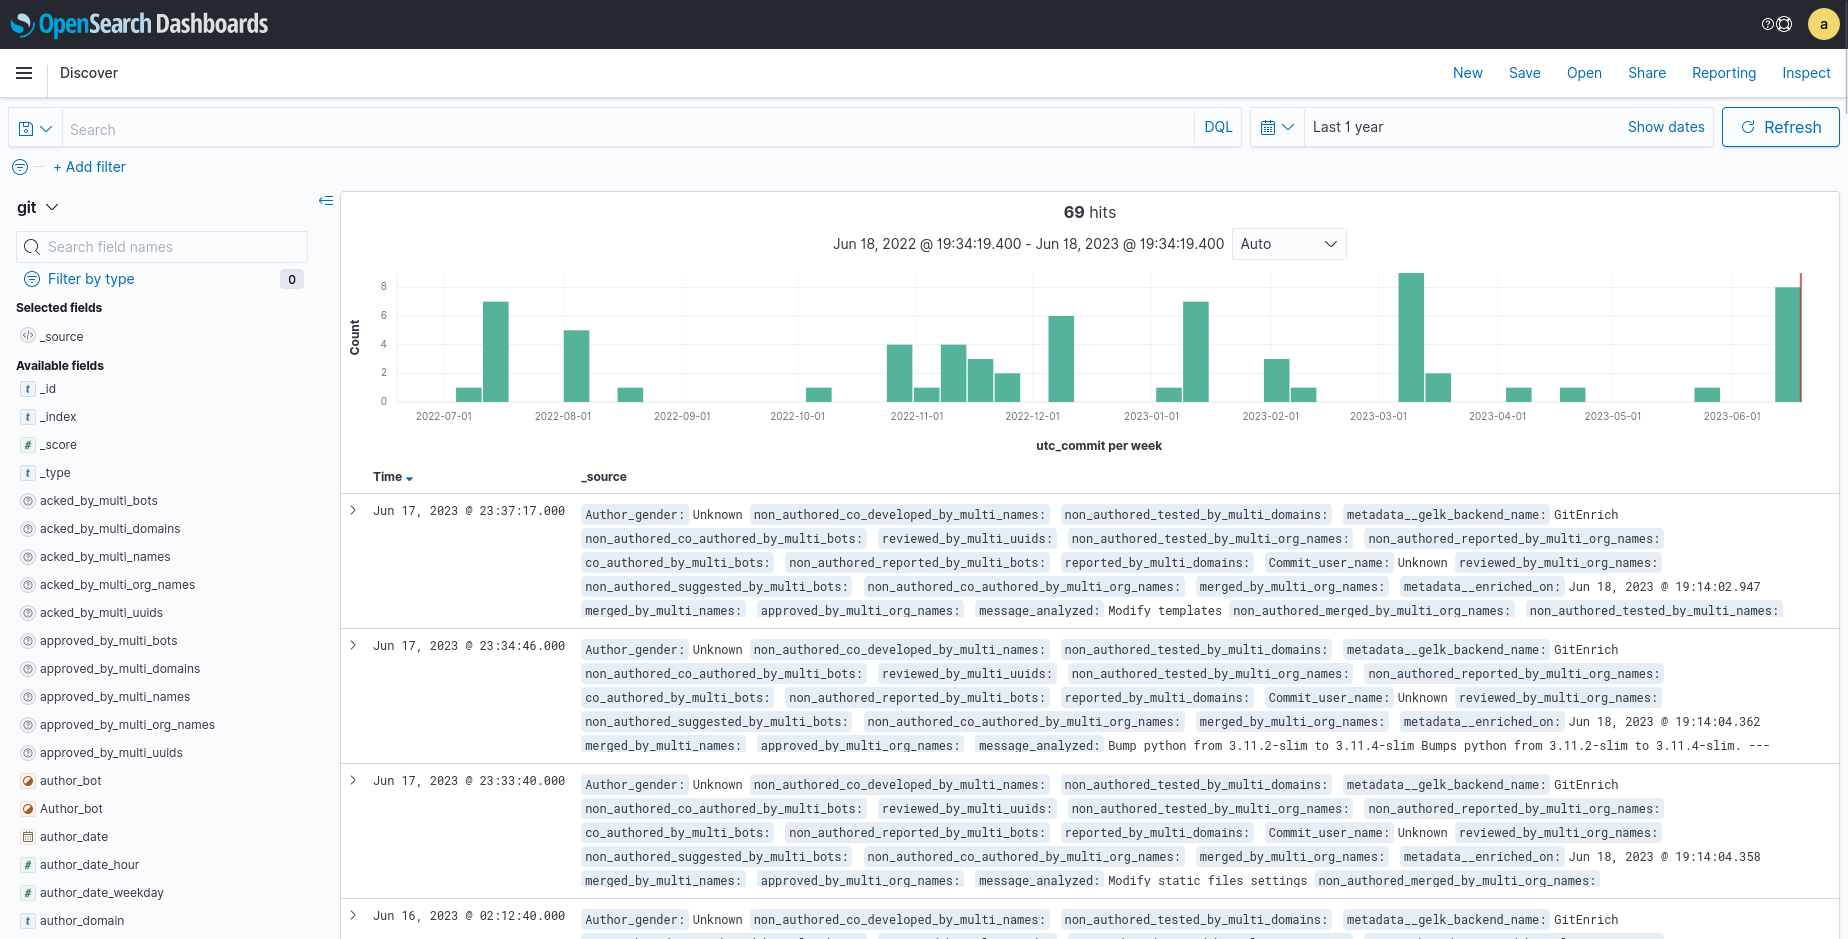
\includegraphics[width=\textwidth]{Figures/opensearch-discover.png}
    \decoRule
    \caption[OpenSearch (Sección \emph{Discover})]{Sección \emph{Discover} en OpenSearch}
    \label{fig:opensearch-discover}
\end{figure}

%% Chapter 1: Last Conclusions

\chapter{Conclusiones} % Main chapter title

\label{Chapter5} % For referencing the chapter elsewhere, use \ref{Chapter5}

%----------------------------------------------------------------------------------------

\section{Consecución de objetivos}

Los objetivos propuestos al comienzo del proyecto eran:

\begin{itemize}
    \item Desarrollar un sistema que genere informes inalterables, creando un flujo más simple desde la solicitud por parte del usuario al \emph{output} de la aplicación.
    \item Desarrollar varios componentes \emph{software}\index{software} independientes que colaboren entre ellos para dar un servicio al usuario.
    \item Simplificar el uso de GrimoireLab\index{GrimoireLab} mediante la ejecución del contenedor Docker\index{Docker} original de GrimoireLab.
    \item Realizar varias mejoras menores respecto a Cauldron\index{Cauldron}.
\end{itemize}

Estos objetivos se han llevado a cabo de manera satisfactoria. El sistema desarrollado permite el análisis de repositorios \emph{software}\index{software} utilizando un esquema de informes inalterables y con una arquitectura descapolada entre sus componentes.

Sin embargo, el objetivo principal que perseguía este proyecto era también el desarrollo de un sistema que mejorase las prestaciones de Cauldron\index{Cauldron}. Este objetivo no se ha cumplido: Cauldron ofrece muchas más características que Grimoirebots a día de hoy, como la existencia de usuarios, la comparación de análisis o un mayor número de fuentes de datos disponible.

%----------------------------------------------------------------------------------------

\section{Conocimientos adquiridos}

Desde la concepción del proyecto hasta la finalización de esta memoria, el autor ha estado inmerso en un continuo aprendizaje. A pesar de tener un conocimiento previo en la mayoría de las tecnologías utilizadas, otras han resultado un descubrimiento y una ampliación en experiencia y sabiduría.

Los conocimientos adquiridos más relevantes son:

\begin{itemize}
    \item Reforzar y ampliar el conocimiento sobre el desarrollo de APIs REST mediante el estudio y uso herramientas novedosas en la creación de APIs REST como Django REST Framework o FastAPI, así como el estudio e investigación del estándar OpenAPI.
    \item Profundizar en el desarrollo de contenedores con Docker, al tener que elaborar esquemas de funcionamiento complejos con estos.
    \item Mejorar la destreza en el desarrollo de código con Python, mediante la escritura de código más limpio y más manejable.
    \item Aprender como funcionan las arquitecturas de \emph{software} con componentes desacoplados, al haber diseñado e implementado los diferentes servicios que componen el sistema.
    \item Ampliar el conocimiento sobre GrimoireLab, mediante el estudio avanzado de todas sus herramientas, su configuración y su ejecución.
    \item Realizar la gestión del tiempo durante el desarrollo del proyecto para cumplir los plazos de entrega.
\end{itemize}

Todo el conocimiento y experiencia adquiridos me ha permitido comprender mejor el mundo del desarrollo web y las arquitecturas de \emph{software} desacopladas. Aunque esperaba haber dotado al sistema de mayor funcionalidad, me quedo con haber sentado las bases de lo que será una gran herramienta para la analítica del desarrollo de \emph{software} en el futuro.

%----------------------------------------------------------------------------------------

\section{Líneas de desarrollo futuras}

Las líneas de desarrollo futuras se centran en mejorar algunas de las prestaciones de Cauldron\index{Cauldron} que se quedaron fuera del alcance original del proyecto.

Utilizar un sistema de colas con prioridades para la realización de los análisis simplificaría bastante el desarrollo necesario para la asignación de tareas, ya que existen componentes creados por terceros pensados para este propósito.

Permitir la creación de usuarios pero, a diferencia de Cauldron\index{Cauldron}, que la autenticación no esté asociada a una fuente de datos, como GitHub\index{GitHub} o Meetup. Django\index{Django} posee un sistema de gestión de usuarios muy sencillo y robusto, y permite extender los modelos básicos con mucha facilidad.

Utilizar y aprovechar las herramientas que ofrecen las plataformas \emph{Cloud} podría mejorar el rendimiento general de la aplicación y reducir sus costes de operación. Servicios y herramientas como \emph{AWS Lambda}, \emph{AWS Fargate}, o \emph{AWS RDS} podrían ser opciones válidas con las especificaciones originales del proyecto.

Desarrollar una interfaz de usuario que facilite el uso del servicio. Para preservar el principio de tener componentes desacoplados, esta interfaz debería ser desarrollada de manera independiente al \emph{backend}, y debería interaccionar con este mediante llamadas a la API\index{} de Grimoirebots. Para hacerlo más interesante, este \emph{frontend} debería diseñarse como un conjunto de páginas estáticas, las cuales conllevan mucho menor gasto operativo, al no necesitar un servidor que procese las solicitudes.

Por último, la inclusión de mecanismos de Integración Continua y Despliegue Continuo permitiría un mayor rendimiento y eficacia en el desarrollo de cada uno de los componentes, al reducir los tiempos de entrega y limitar el error humano.

Todo el código utilizado en este Trabajo de Fin de Máster está disponible en los siguientes repositorios de GitHub\index{GitHub}:

\begin{itemize}
    \item \url{https://github.com/merinhunter/grimoirebots}
    \item \url{https://github.com/merinhunter/grimoirebots-client}
    \item \url{https://github.com/merinhunter/grimoirebots-deployment}
\end{itemize}


%----------------------------------------------------------------------------------------
%	THESIS CONTENT - APPENDICES
%----------------------------------------------------------------------------------------

\appendix % Cue to tell LaTeX that the following "chapters" are Appendices

% Include the appendices of the thesis as separate files from the Appendices folder
% Uncomment the lines as you write the Appendices

% Appendix A

\chapter{Frequently Asked Questions} % Main appendix title

\label{AppendixA} % For referencing this appendix elsewhere, use \ref{AppendixA}

\section{How do I change the colors of links?}

The color of links can be changed to your liking using:

{\small\verb!\hypersetup{urlcolor=red}!}, or

{\small\verb!\hypersetup{citecolor=green}!}, or

{\small\verb!\hypersetup{allcolor=blue}!}.

\noindent If you want to completely hide the links, you can use:

{\small\verb!\hypersetup{allcolors=.}!}, or even better: 

{\small\verb!\hypersetup{hidelinks}!}.

\noindent If you want to have obvious links in the PDF but not the printed text, use:

{\small\verb!\hypersetup{colorlinks=false}!}.

%\include{Appendices/AppendixB}
%\include{Appendices/AppendixC}

%----------------------------------------------------------------------------------------
%	BIBLIOGRAPHY
%----------------------------------------------------------------------------------------

\printbibliography[heading=bibintoc]

%----------------------------------------------------------------------------------------

\end{document}
